\documentclass[a4paper,12pt,openany]{book} % La clase 'book' permite crear libros

\usepackage[utf8]{inputenc}  % Asegura codificación UTF-8
\usepackage{geometry}        % Paquete para configurar márgenes
\geometry{top=0.75in, bottom=0.75in, left=0.75in, right=0.75in}  % Márgenes personalizados
\usepackage{titlesec}        % Personalización de títulos
\usepackage{enumitem}        % Personalización de listas
\usepackage{amsmath}         % Paquete para matemáticas
\usepackage{amsfonts}        % Paquete para fuentes matemáticas
\usepackage{graphicx}        % Paquete para incluir gráficos
\usepackage{hyperref}        % Enlaces y referencias
\usepackage{listings}        % Mostrar código
\usepackage{xcolor}          % Colores para personalizar el código y otros elementos
\usepackage{amsmath, amssymb, amsfonts}
\usepackage{geometry}
\usepackage{lmodern}
\usepackage{multicol}

% Configuración del formato de los títulos
\titleformat{\section}[block]{\normalfont\Large\bfseries}{\thesection}{1em}{}
\titleformat{\subsection}[runin]{\normalfont\bfseries}{\thesubsection}{1em}{}
\titleformat{\subsubsection}[runin]{\normalfont\itshape}{\thesubsubsection}{1em}{}

% Espaciado para los títulos
\titlespacing{\section}{0pt}{12pt}{12pt}
\titlespacing{\subsection}{0pt}{6pt}{6pt}
\titlespacing{\subsubsection}{0pt}{6pt}{6pt}

% Espacio entre párrafos y sin sangría
\setlength{\parskip}{0.5em}  % Espacio entre párrafos
\setlength{\parindent}{0pt}  % Sin sangría en los párrafos

% Cambiar "Chapter" a "Capítulo"
\renewcommand{\chaptername}{Capítulo}
  % Incluye el archivo de configuración

\begin{document}

% CARÁTULA
\title{Guia Ecuaciones Diferenciales - MAT207}
\author{Ing. Luis Antonio Molina Yampa}
\date{25 de Febrero de 2025}
\maketitle  % Genera la carátula

\newpage  % Empieza una nueva página

% LISTA DE CONTENIDOS
\tableofcontents
\cleardoublepage % Aquí se genera la lista de contenidos que incluye las secciones y subsecciones
\newpage  % Empieza una nueva página

% UNIFICACIÓN DE CAPÍTULOS
\chapter{Introducción a las Ecuaciones Diferenciales}

\section{Definición de una Ecuación Diferencial}
Una ecuación diferencial es una ecuación que involucra una función desconocida y sus derivadas. Su importancia radica en que modelan diversos fenómenos en física, biología, economía e ingeniería.

\subsection*{Ejemplo 1.1: Ecuación Diferencial Básica}
Considere la ecuación diferencial:

\begin{equation}
\frac{dy}{dx} = 3x^2
\end{equation}

Para resolverla, integramos ambos lados:

\begin{equation}
y = \int 3x^2 dx = x^3 + C
\end{equation}

donde \( C \) es la constante de integración.

\section{Clasificación de las Ecuaciones Diferenciales}
Las ecuaciones diferenciales se clasifican según distintos criterios:

\subsection{Ecuaciones Diferenciales Ordinarias (EDO)}
Cuando una ecuación involucra una función de una sola variable independiente y sus derivadas.

\subsection{Ecuaciones Diferenciales Parciales (EDP)}
Si la ecuación involucra derivadas parciales de una función con respecto a más de una variable independiente.

\subsection*{Ejemplo 1.2: EDO vs. EDP}
\begin{itemize}
    \item EDO: \( \frac{d^2y}{dx^2} + 4\frac{dy}{dx} + y = 0 \)
    \item EDP: \( \frac{\partial^2 u}{\partial x^2} + \frac{\partial^2 u}{\partial y^2} = 0 \) (Ecuación de Laplace)
\end{itemize}

\section{Orden y Grado de una Ecuación Diferencial}
El \textbf{orden} de una ecuación diferencial es el de la derivada más alta presente en la ecuación.  
El \textbf{grado} es el exponente de la derivada de orden más alto (si está escrita en forma polinómica).

\subsection*{Ejemplo 1.3: Determinación del Orden y Grado}
Dada la ecuación:

\begin{equation}
\left( \frac{d^2y}{dx^2} \right)^3 + 4\frac{dy}{dx} + y = 0
\end{equation}

\begin{itemize}
    \item \textbf{Orden}: 2 (porque la derivada más alta es \( \frac{d^2y}{dx^2} \))
    \item \textbf{Grado}: 3 (porque la derivada de orden 2 está elevada al cubo)
\end{itemize}

\section{Soluciones de una Ecuación Diferencial}
Existen dos tipos principales de soluciones:

\subsection{Solución General}
Contiene una familia de soluciones dependientes de constantes arbitrarias.

\subsubsection*{Ejemplo 1.4}
Resolver \( \frac{dy}{dx} = 2x \):

\begin{equation}
y = \int 2x dx = x^2 + C
\end{equation}

\subsection{Solución Particular}
Se obtiene al asignar valores específicos a las constantes.

Si se da la condición inicial \( y(1) = 5 \):

\begin{equation}
5 = 1^2 + C \Rightarrow C = 4
\end{equation}

Entonces, la solución particular es \( y = x^2 + 4 \).

\section{Ejercicios}
Resuelve los siguientes ejercicios determinando el orden y grado de cada ecuación:

\begin{enumerate}
    \item \( \frac{d^2y}{dx^2} + 5\frac{dy}{dx} + 6y = 0 \)
    \item \( \left( \frac{dy}{dx} \right)^2 + y = x \)
    \item \( \frac{d^3y}{dx^3} + 2\frac{d^2y}{dx^2} + y = 0 \)
    \item \( \left( \frac{d^2y}{dx^2} \right)^{5} + \frac{dy}{dx} = x^3 \)
    \item \( \frac{\partial u}{\partial x} + \frac{\partial u}{\partial y} = 0 \) (Indica si es EDO o EDP)
    \item \( \frac{dy}{dx} = e^x \)
    \item \( \frac{d^2y}{dx^2} + y^2 = 0 \)
    \item \( x^2\frac{d^3y}{dx^3} + x\frac{d^2y}{dx^2} + y = 0 \)
    \item \( \left( \frac{d^2y}{dx^2} \right) + 3 \frac{dy}{dx} + y = x^2 + 1 \)
    \item \( \left( \frac{d^3y}{dx^3} \right)^2 + y = 0 \)
\end{enumerate}

  % Incluye el contenido del capítulo 1
\clearpage
\thispagestyle{plain}
\newpage

\chapter{Ecuaciones Diferenciales Ordinarias de Prmer Orden}
\section{Introducción}
Las ecuaciones diferenciales de primer orden son aquellas en las que la derivada de mayor orden es la primera derivada de la función incógnita. Estas ecuaciones aparecen en una gran variedad de aplicaciones en la física, biología, economía e ingeniería.

\section{Ecuaciones de Variables Separables}
Una ecuación diferencial de primer orden se dice separable si puede escribirse en la forma:

\begin{equation}
\frac{dy}{dx} = g(x)h(y)
\end{equation}

Reescribiéndola:

\begin{equation}
\frac{dy}{h(y)} = g(x)dx
\end{equation}

Al integrar ambos lados:

\begin{equation}
\int \frac{dy}{h(y)} = \int g(x)dx
\end{equation}

\textbf{Metodo Variable Separable}

Considere que para resolver este tipo de ejercicios, la E.D. de ser posible separarla en sus variables, para ello es necesario que este presente en la siguiente forma:


\begin{gather}
\frac{dy}{dx} \ =\ f( x,y) \ \ ( A) \ Estandar\\
\frac{dy}{dx} \ =\ A( x) *B( y) \ \ o\ A( x) /B( y) \  \notag\\
 \notag\\
 \notag\\
M( x,y) dx\ +\ N( x,y) dy\ =\ 0\ \ ( B) \ Diferencial\\
A( x) dx\ +\ B( y) dy\ =\ 0 \notag\\
\int A( x) dx\ +\ \int B( y) dy\ =\ 0 \notag\\
 \notag\\
 \notag
\end{gather}

\subsection*{Ejemplo 1 : Resolución de una ecuación separable sencilla}
Resolver \( \frac{dy}{dx} = x y \).
Separando variables:
\begin{equation}
\frac{dy}{y} = x dx
\end{equation}
Integrando:
\begin{equation}
\ln |y| = \frac{x^2}{2} + C
\end{equation}

Despejando \( y \):

\begin{equation}
y = e^{\frac{x^2}{2} + C} = Ce^{x^2/2}
\end{equation}


\subsection*{Ejemplo 2}

\begin{gather*}
\frac{dy}{dx} \ =\ -6xy,\ \ \ \ \ y( 0) \ =\ 7\\
\\
\int \frac{1}{y} \ dy\ =\ -\int 6xdx\\
ln( y) \ =\ -6\frac{x^{2}}{2} \ +c\\
Encontramos\ la\ solucion\ General\\
y\ =\ e^{\left( -3x^{2} +c\right)}\\
x^{( a+b) \ } =\ x^{( a) \ } *x^{( b) \ }\\
y\ =\ e^{-3x^{2}} e^{c} \ \ \Longrightarrow \ A\ =e^{c} \ \\
y\ =\ Ae^{-3x^{2}}\\
\\
Encontramos\ la\ solucion\ particular\ para\ y( 0) =7\\
7\ =\ Ae^{-3( 0)^{2}}\\
A\ =\ 7\\
y\ =\ 7e^{-3x^{2}}
\end{gather*}
\subsection*{Ejemplo 3}


\begin{gather*}
( 4-2x) dx-\left( 3y^{2} -5\right) dy\ =\ 0\ \ \ y( 1) =3\\
( 4-2x) dx+\left( 5-3y^{2}\right) dy\ =0\\
\int ( 4-2x) dx+\int \left( 5-3y^{2}\right) dy\ =c\\
4x-2\frac{x^{2}}{2} \ +\ 5y-3\frac{y^{3}}{3} \ =\ c\\
4x-x^{2} +5y-y^{3} \ =\ c\\
\\
Encontramos\ la\ solucion\ particular\ con\ \ y( 1) =3\\
4( 1) -( 1)^{2} +5( 3) -( 3)^{3} \ =\ c\\
c\ =\ -9\\
4x-x^{2} +5y-y^{3} \ =\ -9
\end{gather*}

\subsection{Ejercicios Adicionales}

Resolver las siguientes ecuaciones diferenciales:

\begin{enumerate}
    \item \( \tan x\cdot \sin^{2} y\ dx+\cos^{2} x\cdot \cot y\ dy=0 \), \textbf{Solución:} \( \cot^{2} y=\tan^{2} x+C \).

    \item \( xy'-y=y^{3} \), \textbf{Solución:} \( x=\frac{cy}{\sqrt{1+y^{2}}} \).

    \item \( \sqrt{1+x^{3}}\frac{dy}{dx} =x^{2} y+x^{2} \), \textbf{Solución:} \( 2\sqrt{1+x^{3}} =3\ln (y+1)+C \).

    \item \( e^{2x-y} \ dx+e^{-2x} \ dy=0 \), \textbf{Solución:} \( e^{4x} +2e^{2y} =C \).

    \item \( (x^{2} y-x^{2} +y-1)\ dx+(xy+2x-3y-6)\ dy=0 \), \textbf{Solución:} \( \frac{x^{2}}{2} +3x+y+\ln (x-3)^{10} (y-1)^{3} =C \).

    \item \( e^{x+y}\sin x\ dx+(2y+1)e^{-y^{2}} \ dy=0 \), \textbf{Solución:} \( e^{x} (\sin x-\cos x)-2e^{-y^{2}} =C \).

    \item \( 3e^{x} \cdot \tan y\ dx+(1-e^{x} )\sec^{2} y\ dy=0 \), \textbf{Solución:} \( \tan y=C(1-e^{x} )^{3} \).

    \item \( e^{y}\left(\frac{dy}{dx} +1\right) =1 \), \textbf{Solución:} \( \ln (e^{y} -1)=C-x \).

    \item \( y'=1+x+y^{2} +xy^{2} \), \textbf{Solución:} \( \arctan y-\frac{x^{2}}{2} =C \).

    \item \( y-xy'=a(1+x^{2} y) \), \textbf{Solución:} \( y=\frac{a+cx}{1+ax} \).

\end{enumerate}


\section{Ecuaciones Homogéneas}
En este tipo de ecuaciones es practico buscar la forma de representar la E.D. de la siguiente forma:
\begin{equation*}
\frac{dy}{dx} \ =\ f\left(\frac{x}{y} +o\ \ ...\frac{y}{x}\right)
\end{equation*}
Tras buscar la forma de representar la .E.D en ese esquema, se puede hacer el cambio de una de las variables de la siguiente forma
\begin{gather*}
y\ =vx\ \ \ v\ =\frac{y}{x}\\
\frac{dy}{dx} \ =\ v\ +x\frac{dv}{dx} \ \ \Longrightarrow \ dy\ =\ vdx+xdv\\
\\
o\\
x\ =\ uy\ \ \Longrightarrow \ u\ =\ \frac{x}{y}\\
\frac{dx}{dy} \ =\ u\ +y\frac{du}{dy} \ \ \ \Longrightarrow \ dx\ =udy+ydu
\end{gather*}
\textbf{¿Cómo identificar que una E.D. es homogénea?}

Dada una ecuación diferencial de la forma:
\begin{equation*}
    \frac{dy}{dx} = f(x,y)
\end{equation*}
Incorporamos el operador \(\lambda\) en la función:
\begin{equation*}
    \frac{dy}{dx} = f(\lambda x, \lambda y)
\end{equation*}
El objetivo es hacer desaparecer el operador \(\lambda\) y obtener la expresión original:
\begin{equation*}
    \frac{dy}{dx} = f(x,y)
\end{equation*}

Ahora, consideramos la ecuación diferencial en forma general:
\begin{equation*}
    M(\lambda x, \lambda y) dx + N(\lambda x, \lambda y) dy = 0
\end{equation*}
Factorizamos \(\lambda\) y verificamos que el grado sea el mismo:
\begin{equation*}
    \lambda^n M(x,y) dx + \lambda^n N(x,y) dy = 0
\end{equation*}

\subsection*{ 2.1 Ejercicio}

Resolver la ecuación diferencial:

\[
2xy\frac{dy}{dx} = 4x^{2} + 3y^{2}
\]

Dividiendo entre \( 2xy \):

\[
\frac{dy}{dx} = \frac{4x^{2} + 3y^{2}}{2xy}
\]

Verificamos si la ecuación es homogénea usando \( \lambda \):

\[
\frac{dy}{dx} = \frac{4(\lambda x)^{2} + 3(\lambda y)^{2}}{2\lambda x \lambda y}
\]

\[
\frac{dy}{dx} = \frac{4\lambda^{2} x^{2} + 3\lambda^{2} y^{2}}{2\lambda^{2} xy}
\]

\[
\frac{dy}{dx} = \frac{4x^{2} + 3y^{2}}{2xy} \quad \Rightarrow \quad \text{E.D. Original}
\]

Utilizamos el cambio de variable \( y = vx \), donde \( v = \frac{y}{x} \), y aplicamos la derivada:

\[
\frac{dy}{dx} = v + x\frac{dv}{dx}
\]

Reemplazamos en la ecuación:

\[
v + x\frac{dv}{dx} = \frac{4x^{2} + 3(vx)^{2}}{2xvx}
\]

Alternativamente, reescribimos la ecuación:

\[
\frac{dy}{dx} = \frac{4x^{2}}{2xy} + \frac{3y^{2}}{2xy}
\]

\[
\frac{dy}{dx} = 2\frac{x}{y} + \frac{3}{2}\frac{y}{x}
\]

Sustituyendo \( y = vx \):

\[
v + x\frac{dv}{dx} = 2\frac{1}{v} + \frac{3}{2} v
\]

\[
x\frac{dv}{dx} = 2\frac{1}{v} + \frac{3}{2} v - v
\]

\[
x\frac{dv}{dx} = \frac{2}{v} + \frac{v}{2}
\]

\[
x\frac{dv}{dx} = \frac{4+v^{2}}{2v} \quad \Rightarrow \quad \text{E.D. de Variables Separables}
\]

\[
\frac{2v}{4+v^{2}} dv = \frac{1}{x} dx
\]

\[
\int \frac{2v}{4+v^{2}} dv = \int \frac{1}{x} dx
\]

Asumiendo que \( c = \ln(c) \), se obtiene:

\[
\ln(4+v^{2}) = \ln(x) + \ln(c)
\]

Aplicamos propiedades logarítmicas:

\[
\ln(4+v^{2}) = \ln(cx)
\]

Aplicamos la exponencial:

\[
e^{\ln(4+v^{2})} = e^{\ln(cx)}
\]

\[
4+v^{2} = cx
\]

Reemplazamos \( v = \frac{y}{x} \):

\[
4+\frac{y^{2}}{x^{2}} = cx
\]


\subsection{Ejercicio 2.3}

Resolver la siguiente ecuación diferencial:

\[
(x^{2} +y^{2}) dx + (x^{2} -xy) dy = 0
\]

Expresamos en la forma estándar:

\[
\frac{dy}{dx} = -\frac{x^{2} +y^{2}}{x^{2} -xy}
\]

Sustituyendo \( y = vx \) con \( v = \frac{y}{x} \):

\[
\frac{dv}{dx} x + v = -\frac{x^{2} + v^{2} x^{2}}{x^{2} - x x v}
\]

Factorizando:

\[
\frac{dv}{dx} x + v = -\frac{x^{2} (1 + v^{2})}{x^{2} (1 - v)}
\]

\[
\frac{dv}{dx} x = -\frac{1 + v^{2}}{1 - v} - v
\]

\[
\frac{dv}{dx} x = \frac{- (1 + v^{2}) - v (1 - v)}{1 - v}
\]

\[
\frac{dv}{dx} x = \frac{-1 - v^{2} - v + v^{2}}{1 - v}
\]

\[
\frac{dv}{dx} x = -\frac{1 + v}{1 - v}
\]

Integramos ambos lados:

\[
\int \frac{1 - v}{1 + v} dv = -\int \frac{1}{x} dx
\]

Utilizando fracciones parciales:

\[
\int \left( \frac{1}{1+v} - \frac{v}{1+v} \right) dv = -\int \frac{1}{x} dx
\]




\subsection*{Ejercicios Propuestos}
Resuelve las siguientes ecuaciones homogéneas
\begin{enumerate}
    \item $(4x^{2} +xy-3y^{2} )\,dx+(-5x^{2} +2xy+y^{2} )\,dy=0$
    \item $\frac{dy}{dx} =\frac{y}{x} +\left(\frac{\varphi \left(\frac{y}{x}\right)}{\varphi '\left(\frac{y}{x}\right)}\right)$
    \item $xy'=2(y-\sqrt{xy})$
    \item $\left( x\cos\left(\frac{y}{x}\right) -y\right) dx+x\ dy=0$
    \item $xy'=y+2xe^{-y/x}$
    \item $dy =\left(\frac{y}{x} -\cos^{2}\left(\frac{y}{x}\right)\right) dx$
\end{enumerate}

\section*{Ecuaciones Diferenciales Exactas}

Una ecuación diferencial de la forma:
\[
M(x,y)dx + N(x,y)dy = 0
\]
es \textbf{exacta} si y solo si se cumple la siguiente condición:
\[
\frac{\partial M}{\partial y} = \frac{\partial N}{\partial x}
\]

\subsection*{Método de Solución}

Para resolver ecuaciones diferenciales exactas, se sigue el siguiente procedimiento:

\begin{enumerate}
    \item \textbf{Tomar} \( dg(x,y) = Mdx \) o bien \( dg(x,y) = Ndy \).
    \item \textbf{Integrar} en \( x \) o en \( y \).
    \item \textbf{Derivar} con respecto a la variable opuesta.
    \item \textbf{Igualar} el resultado con \( M \) o \( N \) según corresponda.
    \item \textbf{Resolver} la integral resultante.
\end{enumerate}

\subsection*{Ecuaciones No Exactas}

Cuando la ecuación diferencial no cumple con la condición de exactitud:
\[
\frac{\partial M}{\partial y} \neq \frac{\partial N}{\partial x}
\]
se debe encontrar un \textbf{factor integrante} \( F(x,y) \) que convierta la ecuación en exacta, de tal manera que:

\[
F(x,y) Mdx + F(x,y) Ndy = 0
\]

\subsection*{Cálculo del Factor Integrante}

Dependiendo de si el factor integrante es función de \( x \) o de \( y \), se calcula de la siguiente forma:

\begin{itemize}
    \item \textbf{Si el factor es función de \( x \)}:
    \[
    F(x) = e^{\int P(x) dx}, \quad \text{donde } P(x) = \frac{M_y - N_x}{N}
    \]
    
    \item \textbf{Si el factor es función de \( y \)}:
    \[
    F(y) = e^{\int P(y) dy}, \quad \text{donde } P(y) = \frac{N_x - M_y}{M}
    \]

    \item \textbf{Si el factor es función de ambas variables \( x \) y \( y \)}:  
    Se debe determinar por tanteo o con métodos específicos.
\end{itemize}

\subsection*{Resolución con el Factor Integrante}

Una vez multiplicada la ecuación diferencial por el factor integrante, la ecuación resultante se puede resolver con el método de ecuaciones diferenciales exactas.

\[
   Fi( x,y) M( x,y) dx+Fi( x,y) N( x,y) dy=0\ 
    \]

    
\subsection*{Ejemplo 2.3: Resolviendo una ecuación exacta}


\[
(4x+2y^{2})dx + (4xy)dy = 0
\]

Tomamos la ecuación en la forma:
\[
\frac{\partial g( x,y)}{\partial y} = N( x,y)
\]
Reemplazamos \( N(x,y) \):
\[
\frac{\partial g( x,y)}{\partial y} = 4xy
\]

Pasamos la derivada al otro lado como una integral:
\[
g( x,y) = \int 4xy \, dy
\]
Resolviendo la integral:
\[
g( x,y) = 2xy^{2} + c_{1} + v( x)
\]
donde \( v(x) \) es una función desconocida.

Complementamos con la ecuación:
\[
\frac{\partial g( x,y)}{\partial x} = M( x,y)
\]
Derivamos \( g(x,y) \) con respecto a \( x \):
\[
\frac{\partial}{\partial x} \left( 2xy^{2} + c_{1} + v(x) \right) = 2y^{2} + v'(x)
\]
Igualamos con \( M(x,y) \):
\[
2y^{2} + v'(x) = 4x+ 2y^{2}
\]

Despejamos \( v'(x) \):
\[
v'(x) = 4x
\]
Para encontrar \( v(x) \), integramos:
\[
v( x) = \int 4x dx
\]
\[
v( x) = 2x^{2} + c_{2}
\]

Reemplazamos en la ecuación inicial de \( g(x,y) \):
\[
g( x,y) = 2xy^{2} + c_{1} + v( x)
\]
\[
g( x,y) = 2xy^{2} + c_{1} + 2x^{2} + c_{2}
\]

Por teoría, sabemos que:
\[
g( x,y) = C
\]
Entonces:
\[
2xy^{2} + c_{1} + 2x^{2} + c_{2} = C
\]
Unificando constantes:
\[
K = C - c_{1} - c_{2}
\]
\[
2xy^{2} + 2x^{2} = K
\]

Finalmente, despejamos \( y \):
\[
y = \sqrt{\frac{K - 2x^{2}}{2x}}
\]


\subsection{Ejemplo de Resolución de Ecuaciones No Exactas}

\[
xydx + \left( 2x^{2} +3y^{2} -20\right) dy = 0
\]

\noindent Verificamos si es exacta aplicando la condición:
\[
\frac{\partial M( x,y)}{\partial y} = \frac{\partial N( x,y)}{\partial x}
\]

\noindent Calculamos las derivadas parciales:
\begin{align*}
\frac{\partial M( x,y)}{\partial y} &= \frac{\partial ( xy)}{\partial y} = x, \\
\frac{\partial N( x,y)}{\partial x} &= \frac{\partial ( 2x^{2} +3y^{2} -20)}{\partial x} = 4x.
\end{align*}

\noindent Como \( x \neq 4x \), la ecuación no es exacta. Utilizamos las fórmulas para encontrar factores de integración.

\noindent Primero intentamos con la opción (A):
\begin{align*}
\frac{1}{2x^{2} +3y^{2} -20} ( x-4x) &= \frac{-3x}{2x^{2} +3y^{2} -20}.
\end{align*}

\noindent Como el resultado no es una función exclusiva de \( x \), descartamos esta opción.

\noindent Probamos con la opción (B):
\begin{align*}
\frac{1}{xy} ( x-4x) &= -\frac{3}{y}.
\end{align*}

\noindent Como depende exclusivamente de \( y \), podemos aplicar el siguiente factor integrante:
\begin{align*}
I( x,y) &= e^{-\int h( y) dy} = e^{-\int -\frac{3}{y} dy} = e^{3\ln( y)}.
\end{align*}

\noindent Aplicando propiedades logarítmicas:
\[
I( x,y) = e^{\ln( y^{3})} = y^{3}.
\]

\noindent Multiplicamos la ecuación por el factor integrante:
\[
y^{3} ( xydx + ( 2x^{2} +3y^{2} -20) dy) = 0.
\]

\noindent Ahora verificamos si es exacta:
\begin{align*}
\frac{\partial g( x,y)}{\partial x} &= xy^{4}, \\
g( x,y) &= \int xy^{4} dx = \frac{y^{4} x^{2}}{2} + h( y).
\end{align*}

\noindent Aplicamos la segunda condición:
\begin{align*}
\frac{\partial g( x,y)}{\partial y} &= \frac{\partial}{\partial y} \left( \frac{y^{4} x^{2}}{2} + h( y)\right) = 2x^{2} y^{3} +3y^{5} -20y^{3}, \\
2x^{2} y^{3} + h'( y) &= 2x^{2} y^{3} +3y^{5} -20y^{3}, \\
h'( y) &= 3y^{5} -20y^{3}.
\end{align*}

\noindent Integrando \( h'(y) \):
\begin{align*}
h( y) &= \int ( 3y^{5} -20y^{3}) dy = \frac{1}{2} y^{6} -5y^{4} + c_{1}.
\end{align*}

\noindent Sustituyendo en \( g( x,y) \):
\[
g( x,y) = \frac{y^{4} x^{2}}{2} + \frac{1}{2} y^{6} -5y^{4} + c_{1} = K.
\]

\noindent Definiendo la constante \( c = K - c_{1} \):
\[
\frac{1}{2} x^{2} y^{4} + \frac{1}{2} y^{6} -5y^{4} = c.
\]

\subsection{Ejemplo de Resolución de Ecuaciones No Exactas}
Dada la ecuación:
\[
ydx - xdy = 0.
\]

\noindent Verificamos si es exacta:
\begin{align*}
\frac{\partial M( x,y)}{\partial y} &= 1, & \frac{\partial N( x,y)}{\partial x} &= -1.
\end{align*}

\noindent Aplicamos el factor integrante:
\begin{align*}
\frac{1}{N} ( 1+1) &= -\frac{2}{x}, \\
\frac{1}{M} ( 1+1) &= \frac{2}{y}.
\end{align*}

\noindent Aplicando el factor integrante:
\[
I( x,y) = e^{\int g( x) dx} = e^{-2\int \frac{1}{x} dx} = e^{-2\ln( x)} = x^{-2}.
\]

\noindent Multiplicamos por \( I(x,y) \):
\[
(y dx - x dy) x^{-2} = 0.
\]

\noindent Como ahora la ecuación es exacta, resolvemos:
\begin{align*}
\frac{\partial g( x,y)}{\partial x} &= M( x,y) = yx^{-2}, \\
g( x,y) &= \int yx^{-2} dx + h( x), \\
g( x,y) &= -\frac{y}{x} + h( x).
\end{align*}

\noindent Aplicamos la segunda condición:
\[
\frac{\partial g( x,y)}{\partial y} = N( x,y) = \frac{\partial ( -\frac{y}{x} + h( x))}{\partial y} = -x^{-1}.
\]

\noindent Resolviendo:
\begin{align*}
-\frac{1}{x} + h'( x) &= -\frac{1}{x}, \\
h'( x) &= 0, \\
h( x) &= c_{1}.
\end{align*}

\noindent Finalmente:
\[
g( x,y) = -\frac{y}{x} + c_{1} = K.
\]

\noindent Multiplicamos por \( -1 \):
\[
y = Ax.
\]

\section{Ejercicios Propuestos}

Resolver las siguientes ecuaciones diferenciales en caso de ser exactas:

\begin{enumerate}
    \item \( (2xy - \tan y)dx + (x^2 - x\sec^2 y)dy = 0 \)
    
    \textbf{Respuesta:} \( x^2 y - x \tan y = K \)

    \item \( (\sin x \sin y - x e^y)dy = (e^y + \cos x \cos y)dx \)
    
    \textbf{Respuesta:} \( x e^y + \cos y \sin x = K \)

    \item \( (y + y \cos xy) dx + (x + x \cos xy) dy = 0 \)
    
    \textbf{Respuesta:} \( xy + \sin xy = K \)

    \item \( \left(\frac{y}{x} + 6x\right) dx + (\ln x -2) dy = 0 \)
    
    \textbf{Respuesta:} \( y \ln x + 3x^2 - 2y = K \)

    \item \( (\cos 2y - 3x^2 y^2)dx + (\cos 2y - 2x \sin 2y - 2x^3 y)dy = 0 \)
    
    \textbf{Respuesta:} \( \frac{\sin 2y}{2} + x \cos 2y - x^3 y^2 = c \)

    \item \( e^x (x^2 e^x + e^x + xy + y)dx + (x e^x + y)dy = 0 \)
    
    \textbf{Respuesta:} \( x y e^x + \frac{y^2}{2} + \frac{e^{2x}}{4} (2x^2 - 2x + 3)x = c \)

    \item \( (1 + y^2 + xy^2)dx + (x^2 y + y + 2xy)dx = 0 \)
    
    \textbf{Respuesta:} \( 2x + y^2 (1 + x)^2 = c \)

    \item \( (3x^2 \tan y - \frac{2y^3}{x^3})dx + (x^3 \sec^2 y + 4y^3 - \frac{3y^2}{x^2})dy = 0 \)
    
    \textbf{Respuesta:} \( x^3 \tan y + y^4 + \frac{y^3}{x^2} = c \)

    \item \( (2x + \frac{x^2 + y^2}{x^2 y})dx = \left(\frac{x^2 + y^2}{xy^2}\right) dy \)
    
    \textbf{Respuesta:} \( x^3 y + x^2 - y^2 = cxy \)

    \item \( \left(\frac{\sin 2x}{y} + x\right)dx + \left(y - \frac{\sin^2 x}{y^2}\right)dy = 0 \)
    
    \textbf{Respuesta:} \( \frac{\sin^2 x}{y} + \frac{x^2 + y^2}{2} = c \)

    \item \( \left(-\frac{xy}{\sqrt{1 + x^2}} + 2xy - \frac{y}{x}\right)dx + \left(\sqrt{1 + x^2} + x^2 - \ln x\right)dy = 0 \)
    
    \textbf{Respuesta:} \( y \sqrt{1 + x^2} + x^2 y - y \ln x = c \)
\end{enumerate}



\section{Ecuación Diferencial Lineal de Primer Orden}

Dada una ecuación diferencial lineal de primer orden en su forma estándar:

\[
a_{1}( x)\frac{dy}{dx} + a_{0}( x) y = g( x)
\]

El objetivo inicial es llevarla a su forma simple. Para ello, se puede dividir la expresión entre \( a_{1}( x) \):

\[
\frac{dy}{dx} + \frac{a_{0}( x)}{a_{1}( x)} y = \frac{g( x)}{a_{1}( x)}
\]

Para contextualizar el método, se realiza un pequeño cambio de variables:

\[
P( x) = \frac{a_{0}( x)}{a_{1}( x)}, \quad Q( x) = \frac{g( x)}{a_{1}( x)}
\]

Logrando así la siguiente representación deseada:

\[
\frac{dy}{dx} + P( x) y = Q( x)
\]

Considerando que ahora la ecuación diferencial es lineal, según el método, se procede a aplicar el procedimiento adecuado para su resolución.

\subsubsection{Resolución de una Ecuación Diferencial Lineal Demostracion}

Para resolver una ecuación diferencial lineal, se sigue el siguiente procedimiento:

Identificar un \textbf{factor de integración} \( u(x) \) que nos permita multiplicar la ecuación diferencial:

\[
u( x) y' + u( x) p( x) y = u( x) q( x)
\]

El objetivo de multiplicar por \( u(x) \) es lograr que la ecuación tenga la forma de una derivada de un producto:

\[
(u y)' = u y' + u' y
\]

Comparando términos, se obtiene:

\[
u' = u( x) p( x)
\]

\[
u' = up
\]

\[
\frac{u'}{u} = p
\]

Integrando ambos lados:

\[
\int \frac{u'}{u} dx = \int p dx
\]

\[
\ln u = \int p dx
\]

\[
u = e^{\int p dx}
\]

Así, el factor de integración es:

\[
u( x) = e^{\int p( x) dx}
\]

Multiplicamos la ecuación por \( u(x) \), lo que nos permite escribirla como una derivada exacta:

\[
( u y)' = u( x) q( x)
\]

Integrando en ambos lados:

\[
u y = \int u( x) q( x) dx
\]

Finalmente, despejamos \( y(x) \):

\[
y( x) = u( x)^{-1} \left(\int u( x) q( x) dx + C\right)
\]


\subsubsection{Ejercicio 1}

Resolver la ecuación diferencial:

\[
\frac{dy}{dt} +2y = 4
\]

Identificamos los coeficientes:

\[
p(t) = 2, \quad q(t) = 4
\]

Calculamos el factor de integración:

\[
u(t) = e^{\int 2dt} = e^{2t}
\]

Aplicamos el método:

\[
y(t) = u(t)^{-1} \left(\int u(t) q(t) dt +C\right)
\]

\[
y(t) = e^{-2t} \left(\int 4e^{2t} dt +C\right)
\]

\[
y(t) = e^{-2t} \left( 4\frac{e^{2t}}{2} +C\right)
\]

\[
y(t) = 2 + Ce^{-2t}
\]

---

\subsubsection{Ejercicio 2}

Resolver la ecuación diferencial con la condición inicial \( y(1) = 4 \):

\[
x\frac{dy}{dx} + 2y = 4x^{2}
\]

Reescribimos la ecuación en su forma estándar:

\[
y' + p(x) y = q(x)
\]

Identificamos los coeficientes:

\[
p(x) = 2, \quad q(x) = 4x^2
\]

Para que la ecuación esté correctamente formulada, dividimos entre \( x \):

\[
\frac{dy}{dx} + 2\frac{1}{x} y = 4x, \quad y(1) = 4
\]

Ahora:

\[
p(x) = 2\frac{1}{x}, \quad q(x) = 4x
\]

Calculamos el factor de integración:

\[
u(x) = e^{\int p(x) dx} = e^{2\int \frac{1}{x} dx}
\]

\[
u(x) = e^{2\ln x} = e^{\ln(x^2)}
\]

\[
u(x) = x^2
\]

Multiplicamos la ecuación diferencial por \( u(x) \):

\[
x^{2} \frac{dy}{dx} + 2xy = 4x^{3}
\]

\[
(u(x) \cdot y)' = 4x^{3}
\]

Integrando:

\[
x^{2} y = 4\int x^{3} dx
\]

\[
x^{2} y = 4\frac{x^{4}}{4} +C
\]

\[
y = x^{2} + Cx^{-2}
\]

Usamos la condición inicial \( y(1) = 4 \) para encontrar \( C \):

\[
4 = 1 + C
\]

\[
C = 3
\]

\[
y = x^{2} + 3x^{-2}
\]


\subsection{Ejercicios Propuestos}

Resolver las siguientes ecuaciones diferenciales:

\begin{enumerate}
    \item \( x \tan^2 y \, dy + x \, dy = (2x^2 + \tan y)dx \), \textbf{Respuesta:} \( \tan y = x (2\sin x + c) \).

    \item \( \frac{dy}{dx} - e^x y = \frac{1}{x^2} \sin \frac{1}{x} - e^x \cos \frac{1}{x} \), \textbf{Respuesta:} \( y = \cos \frac{1}{x} + C e^{-x} \).

    \item \( x \sin \theta \, d\theta + (x^3 - 2x^2 \cos \theta + \cos \theta)dx = 0 \), \textbf{Respuesta:} \( \cos \theta = \frac{-x}{2} + C x e^{-x^2} \).

    \item \( x^2 dy + xy dx = 8x^2 \cos^2 x dx \), \textbf{Respuesta:} \( xy = 2x^2 + 2x \sin 2x + \cos 2x + c \).

    \item \( (x^5 + 3y)dx - x dy = 0 \), \textbf{Respuesta:} \( y = x^3 \left(\frac{x^2}{2} + c \right) \).

    \item \( dy = x^{-5} (4x^4 y + 3x^4 y^{-1} + 256y^7 + 768y^5 + 864y^3 + 432y + 81y^{-1})dx \).

    \item \( \frac{dy}{dx} - y \cot x = \frac{\sin(2x)}{2} \), \textbf{Respuesta:} \( y = K \sin x + \sin^2 x \).

    \item \( \cos y \, dx = (x \sin y + \tan y) dy \), \textbf{Respuesta:} \( x = K \sec y - \sec y \ln \cos y \).

\end{enumerate}


\section{Ecuación Diferencial de Bernoulli}

Las ecuaciones de Bernoulli tienen la siguiente representación. A diferencia de una ecuación diferencial lineal, estas cuentan con un término \( y^n \) multiplicando a \( q(x) \):

\[
y' + p(x) y = q(x) y^n
\]

donde \( n \) es un número real diferente de \( 0 \) y \( 1 \).

El objetivo es buscar una forma de convertir la ecuación diferencial en una ecuación lineal.

Para eliminar \( y^n \) en el miembro derecho, dividimos entre \( y^n \):

\[
y^{-n} y' + p(x) y y^{-n} = q(x)
\]

\[
y^{-n} y' + p(x) y^{1-n} = q(x)
\]

Para lograr el formato estándar de una ecuación lineal, realizamos el cambio de variable:

\[
z = y^{1-n} \quad \Rightarrow \quad \text{(A)}
\]

Reemplazando en la ecuación:

\[
y^{-n} y' + p(x) z = q(x)
\]

Buscamos una forma de expresar \( y^{-n} y' \) en términos de \( z' \), es decir, \( \frac{dz}{dx} \).

Derivamos la ecuación (A):

\[
\frac{dz}{dy} = (1 - n) y^{-n}
\]

Aplicamos la regla de la cadena para incorporar \( dx \):

\[
\frac{dz}{dy} = (1 - n) y^{-n} \frac{dx}{dx}
\]

Esto permite separar las variables:

\[
\frac{dz}{dx} = (1 - n) y^{-n} \frac{dy}{dx}
\]

Para aplicar este cambio en la ecuación original, multiplicamos por \( (1 - n) \):

\[
(1 - n) y^{-n} y' + (1 - n) p(x) z = (1 - n) q(x)
\]

\[
z' + (1 - n) p(x) z = (1 - n) q(x)
\]

Esta es una ecuación diferencial lineal en términos de \( z \), que puede resolverse con el método estándar.



\subsection* {Ejercicios 1.2}


Resolver la ecuación diferencial:

\[
2xy \frac{dy}{dx} = 4x^2 + 3y^2
\]

Reordenamos:

\[
2xy \frac{dy}{dx} - 4x^2 = 3y^2
\]

Dividimos entre \( 2xy \):

\[
\frac{dy}{dx} - 2x \frac{1}{y} = \frac{3}{2x} y
\]

Forma de Bernoulli:

\[
y' - \frac{3}{2x} y = 2x y^{-1}, \quad n = -1
\]

Realizamos el cambio de variable:

\[
z = y^{1-n} = y^2
\]

Derivamos:

\[
\frac{dz}{dx} = 2y \frac{dy}{dx}
\]

Multiplicamos por \( (1-n) = 2 \):

\[
2yy' - \frac{3}{x} y^2 = 4x
\]

\[
z' - \frac{3}{x} z = 4x
\]

Factor de integración:

\[
u(x) = e^{\int -\frac{3}{x} dx} = e^{-3\ln x} = x^{-3}
\]

Resolviendo:

\[
z(x) = x^3 \left(\int 4x^{-2} dx + C\right)
\]

\[
z(x) = x^3 \left(-4x^{-1} + C\right)
\]

Reemplazamos \( z = y^2 \):

\[
y^2 = x^3 \left(-4x^{-1} + C\right)
\]

\[
y^2 = Cx^3 - 4x^2
\]

---

\subsection* {Ejercicios 1.3}

Resolver la ecuación diferencial:

\[
x \frac{dy}{dx} + 6y = 3x y^{4/3}
\]

Dividimos entre \( x \):

\[
\frac{dy}{dx} + \frac{6}{x} y = 3y^{4/3}
\]

Dividimos entre \( y^{4/3} \), con \( n = 4/3 \):

\[
y^{-4/3} \frac{dy}{dx} + \frac{6}{x} y^{-1/3} = 3
\]

Cambio de variable:

\[
z = y^{1-n} = y^{-1/3}
\]

Derivamos y aplicamos la regla de la cadena:

\[
\frac{dz}{dx} = -\frac{1}{3} y^{-4/3} \frac{dy}{dx}
\]

Multiplicamos por \( -\frac{1}{3} \):

\[
\frac{dz}{dx} - \frac{2}{x} z = -1
\]

Ecuación diferencial lineal con:

\[
p(x) = -\frac{2}{x}, \quad q(x) = -1
\]

Factor de integración:

\[
u(x) = e^{\int -\frac{2}{x} dx} = x^{-2}
\]

Resolviendo para \( z(x) \):

\[
z(x) = x^2 \left(-\int x^{-2} dx + C\right)
\]

\[
z(x) = x^2 \left(x^{-1} + C\right)
\]

Reemplazamos \( z = y^{-1/3} \):

\[
y^{-1/3} = x^2 \left(x^{-1} + C\right)
\]

---

\subsection* {Ejercicios 1.4 - Casos especiales}

Resolver la ecuación diferencial:

\[
2x e^{2y} \frac{dy}{dx} = 3x^4 + e^{2y}
\]

Intentamos separación de variables:

\[
\frac{dy}{dx} = \frac{3x^4 + e^{2y}}{2x e^{2y}}
\]

No es posible separar, verificamos homogeneidad:

\[
\frac{dy}{dx} = \frac{3 \lambda^4 x^4 + e^{2y \lambda}}{2x \lambda e^{2y \lambda}}
\]

Forma diferencial:

\[
(3x^4 + e^{2y}) dx - 2x e^{2y} dy = 0
\]

No es exacta. Intentamos el cambio:

\[
z = e^{2y}
\]

Derivamos:

\[
\frac{dz}{dx} = 2e^{2y} \frac{dy}{dx}
\]

Sustituyendo en la ecuación:

\[
x \frac{dz}{dx} = 3x^4 + z
\]

Dividimos entre \( x \):

\[
\frac{dz}{dx} = 3x^3 + \frac{1}{x} z
\]

La ecuación se vuelve lineal:

\[
\frac{dz}{dx} - \frac{1}{x} z = 3x^3
\]

\[
p(x) = -\frac{1}{x}, \quad q(x) = 3x^3
\]

---

\subsection* {Ejercicios 1.5}

\[
x e^y \frac{dy}{dx} = 2(e^y + x^3 e^{2x})
\]

\textbf{Solución:}

\[
y = \ln \left( Cx^2 + x^2 e^{2x} \right)
\]

\subsection{Ejercicios Propuestos}

Resolver las siguientes ecuaciones diferenciales:

\begin{enumerate}
    \item \( (x^2 + y^2 + 1)dy + xy dx = 0 \), \textbf{Respuesta:} \( y^4 + 2x^2 y^2 + 2y^2 = K \).

    \item \( \frac{dy}{dx} + \frac{y}{x+1} = -\frac{1}{2}(x+1)^3 y^2 \), \textbf{Respuesta:} \( \frac{1}{y^2} = \frac{(x+1)^4}{2} + C(x+1)^2 \).

    \item \( (x^2 + 1)y' = xy + x^2 y^2 \), \textbf{Respuesta:} \( \frac{1}{y} = \frac{1}{\sqrt{1+x^2}} \left(-\frac{1}{2} \ln |x + \sqrt{1+x^2}| - x \sqrt{1+x^2} + c \right) \).

    \item \( \frac{dy}{dx} = \frac{4 \sin^2 y}{x^5 + x \tan y} \), \textbf{Respuesta:} \( x^4(K - \ln \tan y) = \tan y \).

    \item \( (x^2 + y^2 + (y + 2x)x^{-1}) dy = (2(x^2 + y^2) + (y + 2x)x^{-2}y)dx \),  
    \textbf{Respuesta:} \( (y - 2x)^2 = -\frac{2y}{x} + 10 \arctan \frac{y}{x} \), \textbf{Sugerencia:} \( y = ux \).

    \item \( (xy^2)' = (xy)^3 (x^2 + 1) \), \textbf{Respuesta:} \( y = \frac{45}{45 \sqrt{x} - 5x^5 - 9x^3} \).

    \item \( dy - y \sin x \,dx = y \ln(y e^{\cos x})dx \), \textbf{Respuesta:} \( y = -e^{x - \cos x} \).

    \item \( (x + y^3) + 6xy^2 y' = 0 \), \textbf{Respuesta:} \( y^3 = -\frac{x}{3} + C \frac{1}{2} \).

\end{enumerate}

  % Incluye el contenido del capítulo 2
\clearpage
\thispagestyle{plain}
\newpage

\chapter{Aplicaciones de Modelado para Ecuaciones Diferenciales de Primer Orden}
\section{Introducción}
Las ecuaciones diferenciales de primer orden aparecen en una gran variedad de problemas del mundo real. 
Se utilizan para modelar fenómenos en la física, biología, economía, ingeniería y otras disciplinas.
En este capítulo, se explorarán diversas aplicaciones del modelado con ecuaciones diferenciales de primer orden.


\section{Interés Compuesto Continuo}

Una persona deposita \$5000 en su cuenta con interés compuesto continuo. Suponiendo que no hay depósitos adicionales ni retiros, ¿cuánto dinero habrá en la cuenta después de 7 años si la tasa de interés es constante del 8.5\% durante los primeros 4 años y del 9.25\% durante los últimos 3 años?

La fórmula del interés compuesto continuo es:

\[
P = A e^{kt}
\]

Dado que inicialmente el monto es:

\[
P_0 = 5000, \quad t_0 = 0
\]

Determinamos el modelo inicial:

\[
5000 = A e^{k(0)}
\]

\[
A = 5000
\]

Sustituyendo en la fórmula:

\[
P_1 = 5000 e^{kt}
\]

Para los primeros 4 años, con \( k = 0.085 \):

\[
P_1 = 5000 e^{0.085(4)}
\]

\[
P_1 = 7024.74
\]

Para los siguientes 3 años, usamos la misma ecuación:

\[
P_2 = A e^{0.0925 t}
\]

En el punto de 4 años, recalculamos \( A \):

\[
P_2 = 7024.74, \quad t_2 = 4
\]

\[
7024.74 = A e^{0.0925(4)}
\]

\[
A = \frac{7024.74}{e^{0.0925(4)}} = 4852.23
\]

Por lo tanto, la solución a la ecuación diferencial bajo estas condiciones es:

\[
P_2 = 4852.23 e^{0.0925 t}
\]

Para calcular el monto en el año 7:

\[
P_2 = 4852.23 e^{0.0925(7)}
\]

\[
P_2 = 9271.44
\]

\subsection{Representación Gráfica}
\noindent
\begin{figure}[H]
    \centering
    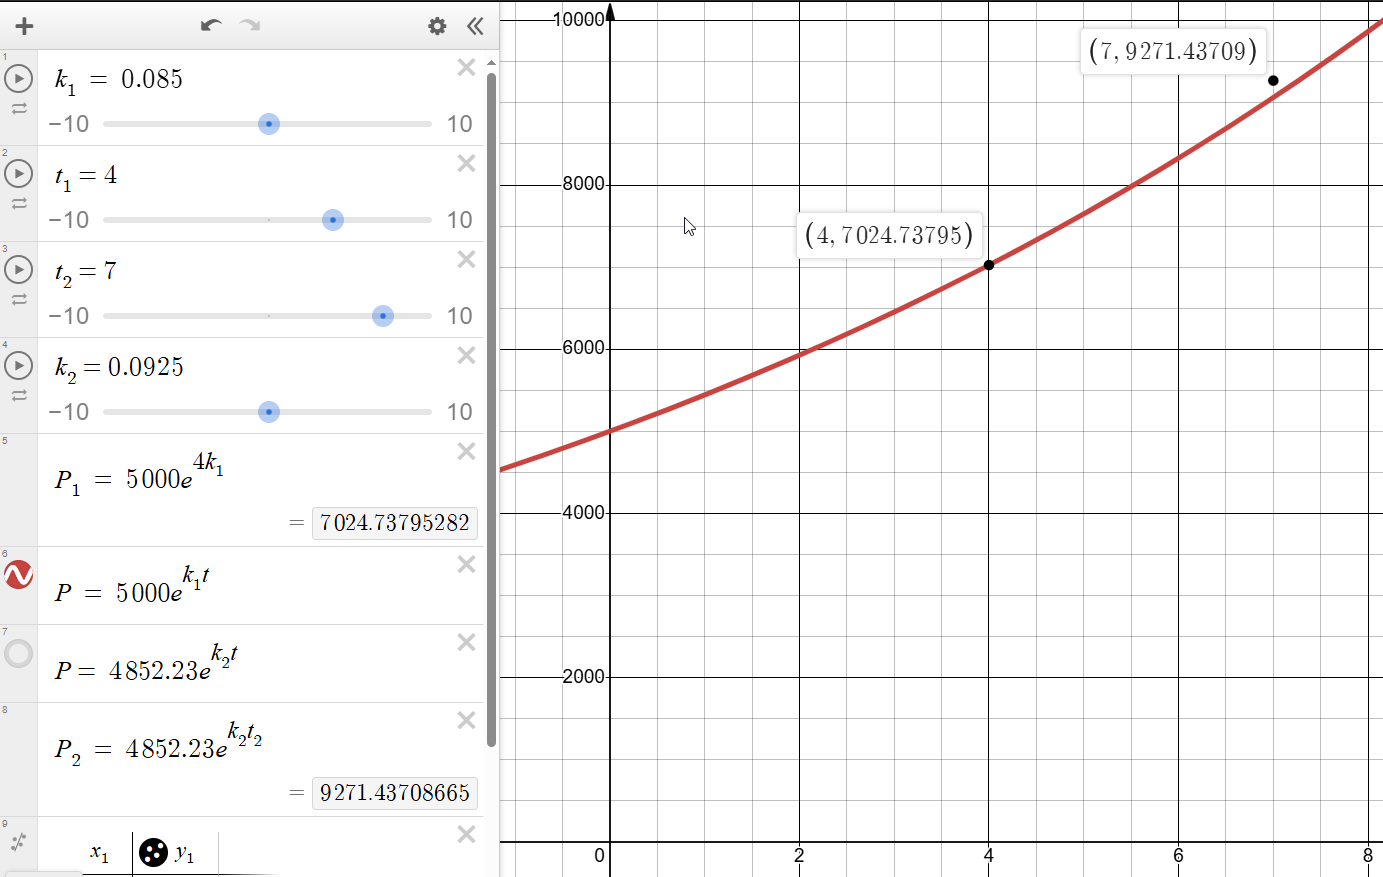
\includegraphics[width=0.6\textwidth]{images/Modelado 01.png}
    \caption{Modelo de interés compuesto continuo}
    \label{fig:modelo-interes}
\end{figure}


\section*{Ejercicio 1: Crecimiento de una Población de Bacterias}

Un determinado estudio de bacterias inicialmente tiene una población \( P_{0} \). Tras haber transcurrido 1 hora, el número de bacterias aumentó a \( \frac{3}{2} P_{0} \). 

Si la tasa de crecimiento es proporcional al número de bacterias presentes en un tiempo \( t \), determina el tiempo necesario para que la población de bacterias triplique su valor.

\begin{figure}[H]
    \centering
    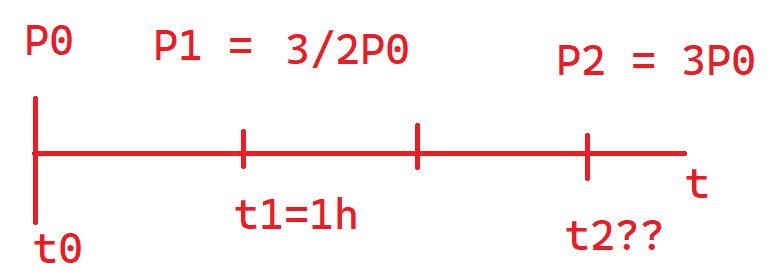
\includegraphics[width=0.7\textwidth]{images/Modelado 02.png}
    \caption{Representación del problema de crecimiento bacteriano}
\end{figure}

La ecuación diferencial que modela el problema es:

\[
\frac{dP}{dt} = kP
\]

Resolviendo:

\[
\int \frac{1}{P} dP = \int k dt
\]

\[
\ln(P) = kt + c
\]

\[
P = e^{kt+c}
\]

\[
P = A e^{kt}, \quad \text{donde } A = e^c
\]

Utilizando los datos iniciales:

\[
P(0) = P_{0} \Rightarrow P_{0} = A e^{k(0)}
\]

\[
A = P_{0}
\]

Para \( P(1) = \frac{3}{2} P_{0} \):

\[
\frac{3}{2} P_{0} = P_{0} e^{k(1)}
\]

\[
\frac{3}{2} = e^k
\]

\[
k = \ln\left(\frac{3}{2}\right) = 0.40
\]

Para determinar \( t_2 \) donde \( P(t_2) = 3P_{0} \):

\[
3 P_{0} = P_{0} e^{0.4t_{2}}
\]

\[
3 = e^{0.4t_{2}}
\]

\[
t_{2} = \frac{\ln(3)}{\ln\left(\frac{3}{2}\right)} = 2.71
\]

Si la población inicial fuera 100 bacterias:

\begin{figure}[H]
    \centering
    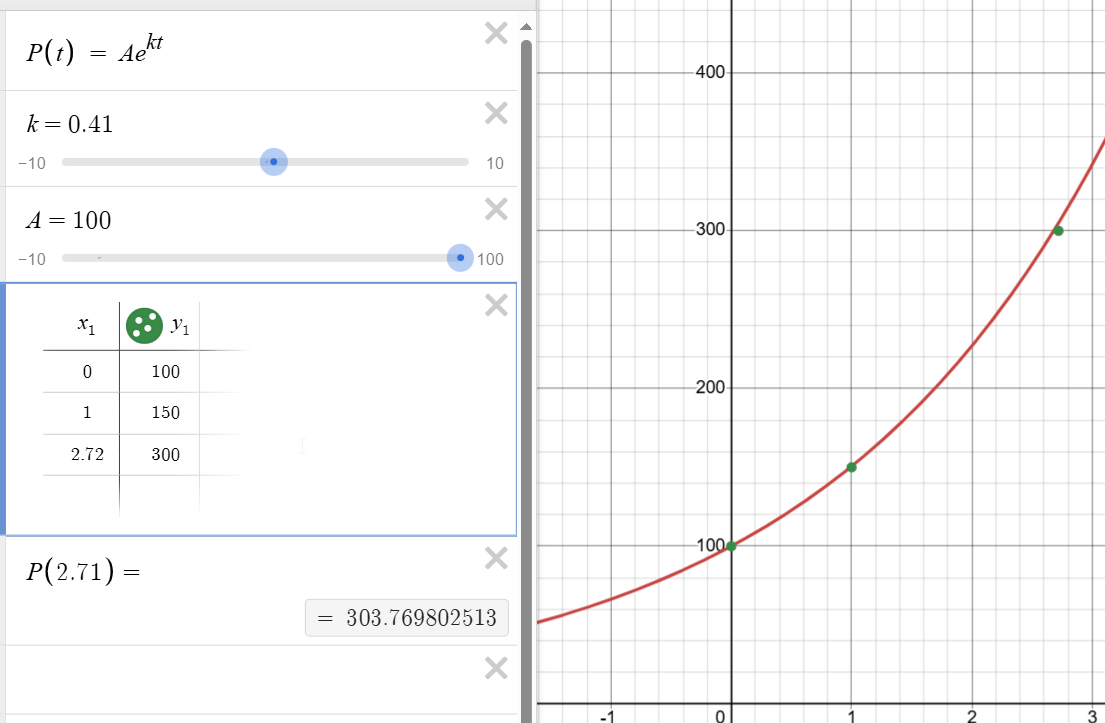
\includegraphics[width=0.7\textwidth]{images/Modelado 03.png}
    \caption{Simulación con población inicial de 100}
\end{figure}

---

\section*{Ejercicio 2: Crecimiento de una Colonia de Bacterias}

Se sabe que inicialmente la población era de 1000 bacterias y que tras 1 hora se duplicó. Se pide:

1. Determinar la ecuación diferencial particular.
2. Calcular la población tras 1.5 horas.

\begin{figure}[H]
    \centering
    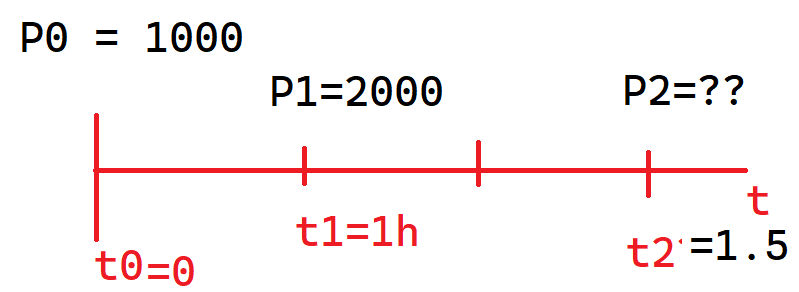
\includegraphics[width=0.7\textwidth]{images/Modelado 04.png}
    \caption{Representación del problema de crecimiento bacteriano}
\end{figure}

Datos:

\[
P(0) = 1000, \quad P(1) = 2000
\]

Usando la ecuación:

\[
P(t) = A e^{kt}
\]

\[
1000 = A e^{k(0)}
\]

\[
A = 1000
\]

\[
2000 = 1000 e^{k(1)}
\]

\[
2 = e^k \Rightarrow k = \ln(2)
\]

\[
P(t) = 1000 e^{\ln(2) t}
\]

Para \( P(1.5) \):

\[
P(1.5) = 1000 e^{\ln(2)(1.5)}
\]

\[
P(1.5) = 2828
\]

---

\section*{Ejercicio 3: Decaimiento Radioactivo}

Un material radioactivo pierde masa de manera proporcional a su cantidad presente. Se sabe que inicialmente había 50 mg y que tras 2 horas perdió el 10\% de su masa. Se pide:

1. Determinar una ecuación para la masa remanente.
2. Calcular la masa tras 4 horas.
3. Encontrar el tiempo en que la masa se reduce a la mitad.

\begin{figure}[H]
    \centering
    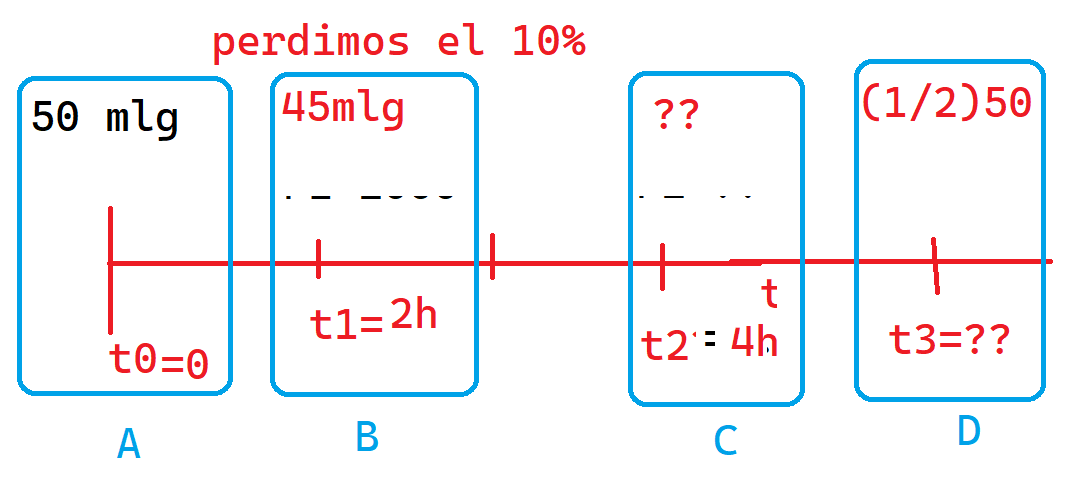
\includegraphics[width=0.7\textwidth]{images/Modelado 05.png}
    \caption{Curva de decaimiento del material radioactivo}
\end{figure}


\section*{Ejercicio 4: Enfriamiento de una Barra de Metal}

Una barra de metal con temperatura inicial de 100ºF es colocada en un ambiente con temperatura constante de 0ºF. Después de 20 minutos, su temperatura se reduce a 50ºF. Se pide:

1. Determinar el tiempo para alcanzar 25ºF.
2. Calcular la temperatura tras 10 minutos.

El problema sigue la **Ley de Enfriamiento de Newton**:

\[
\frac{dT}{dt} = -k(T - T_{\infty})
\]

\section{Crecimiento Poblacional: Modelo Logístico}
El crecimiento poblacional puede modelarse mediante la ecuación diferencial:

\begin{equation}
\frac{dP}{dt} = r P \left( 1 - \frac{P}{K} \right)
\end{equation}

donde \( P(t) \) es la población en el tiempo \( t \), \( r \) es la tasa de crecimiento y \( K \) es la capacidad de carga del entorno.

\subsection*{Ejemplo 3.1: Modelado del Crecimiento Poblacional}
Supongamos que una población de conejos sigue el modelo logístico con \( r = 0.1 \) y \( K = 500 \). Si inicialmente hay 50 conejos, determinar la ecuación de crecimiento.

\subsection*{Ejercicios}
\begin{enumerate}
    \item Resolver el modelo logístico para \( r = 0.2 \), \( K = 1000 \) con una población inicial de 100.
\end{enumerate}

\section{Caída Libre con Resistencia del Aire}
La ecuación de movimiento de un objeto en caída libre con resistencia del aire es:

\begin{equation}
m \frac{dv}{dt} = mg - kv
\end{equation}

donde \( v \) es la velocidad, \( m \) la masa, \( g \) la gravedad y \( k \) el coeficiente de resistencia.

\subsection*{Ejemplo 3.2: Cálculo de Velocidad con Resistencia del Aire}
Determinar la velocidad terminal de un paracaidista de 80 kg con un coeficiente de resistencia \( k = 10 \).

\subsection*{Ejercicios}
\begin{enumerate}
    \item Resolver la ecuación de caída libre para \( k = 5 \) y \( m = 60 \).
\end{enumerate}

\section{Enfriamiento de Newton}
El modelo de enfriamiento de Newton se expresa como:

\begin{equation}
\frac{dT}{dt} = -k (T - T_a)
\end{equation}

donde \( T \) es la temperatura del objeto, \( T_a \) la temperatura ambiente y \( k \) la constante de enfriamiento.

\subsection*{Ejemplo 3.3: Enfriamiento de un Café}
Un café a 90°C se enfría en una habitación a 20°C. Si \( k = 0.02 \), encontrar la temperatura en 10 minutos.

\subsection*{Ejercicios}
\begin{enumerate}
    \item Resolver para un objeto que comienza a 100°C en un ambiente de 30°C con \( k = 0.015 \).
\end{enumerate}

\section{Crecimiento y Desintegración Radiactiva}
La desintegración radiactiva se modela como:

\begin{equation}
\frac{dN}{dt} = -\lambda N
\end{equation}

donde \( N \) es la cantidad de sustancia y \( \lambda \) la constante de desintegración.

\subsection*{Ejemplo 3.4: Desintegración del Carbono-14}
El carbono-14 tiene una vida media de 5730 años. Encontrar la ecuación de desintegración.

\subsection*{Ejercicios}
\begin{enumerate}
    \item Determinar la cantidad restante de una muestra de 100 mg de uranio-238 después de 1000 años.
\end{enumerate}

\section{Dinámica de Enfermedades Infecciosas}
El modelo SIR para la propagación de enfermedades es:

\begin{equation}
\frac{dS}{dt} = -\beta SI, \quad \frac{dI}{dt} = \beta SI - \gamma I
\end{equation}

donde \( S \) es la población susceptible, \( I \) la infectada, \( \beta \) la tasa de transmisión y \( \gamma \) la tasa de recuperación.

\subsection*{Ejemplo 3.5: Propagación de un Virus}
Simular una epidemia con \( \beta = 0.3 \) y \( \gamma = 0.1 \) en una población de 1000 personas.

\subsection*{Ejercicios}
\begin{enumerate}
    \item Resolver el modelo SIR con \( \beta = 0.2 \) y \( \gamma = 0.05 \).
\end{enumerate}

\section{Modelos de Interés Compuesto}
El modelo de interés compuesto se describe como:

\begin{equation}
\frac{dA}{dt} = r A
\end{equation}

donde \( A \) es la cantidad de dinero e \( r \) la tasa de interés.

\subsection*{Ejemplo 3.6: Crecimiento de una Inversión}
Calcular el crecimiento de una inversión inicial de \$1000 con \( r = 5\% \) anual.

\subsection*{Ejercicios}
\begin{enumerate}
    \item Resolver para \( r = 3\% \) con una inversión de \$5000.
\end{enumerate}

\section{Regulación de la Glucosa en la Sangre}
El modelo de control de insulina se expresa como:

\begin{equation}
\frac{dG}{dt} = -k G + I
\end{equation}

donde \( G \) es el nivel de glucosa y \( I \) la insulina inyectada.

\subsection*{Ejemplo 3.7: Control de Glucosa}
Modelar la respuesta del cuerpo a una inyección de insulina con \( k = 0.1 \).

\subsection*{Ejercicios}
\begin{enumerate}
    \item Resolver para \( k = 0.05 \) con una dosis de insulina de 10 unidades.
\end{enumerate}

  % Incluye el contenido del capítulo 3
\clearpage
\thispagestyle{plain}
\newpage

\chapter{Ecuaciones Diferenciales de Orden Superor}
\section{Introducción}
Las ecuaciones diferenciales de orden superior son fundamentales en el estudio de la dinámica de sistemas físicos, eléctricos y mecánicos. En este capítulo exploraremos métodos analíticos para resolverlas, así como sus aplicaciones.

\section{Nomenclatura}
\vspace{-20pt} % Adjust as needed
\begin{align*}
 & \textit{}{Primera Derivada:} \quad y'=\frac{dy}{dx}\\
 & \textit{Segunda Derivada:} \quad y''=\frac{d^{2} y}{dx^{2}}\\
 & \textit{Tercera Derivada:} \quad y'''=\frac{d^{3} y}{dx^{3}}\\
 & \textit{Cuarta Derivada:} \quad y^{(4)} =\frac{d^{4} y}{dx^{4}} \quad (\text{diferente de } y^4 \text{ (potencia)})\\
 & \textbf{Derivada de orden superior:} \quad y^{(n)} =\frac{d^{n} y}{dx^{n}}
\end{align*}


\section{Ecuaciones Diferenciales de Orden Superior Lineales}

\subsection{Clasificación}

Según los coeficientes (funciones de \( x \)) que multiplican a las diferenciales y la variable dependiente:

\subsubsection{E.D. con coeficientes constantes}  
\[
a( x) y''+ b( x) y'+ c( x) y=\ g( x)
\]
Ejemplo:
\[
y''+5y'+3y\ =\ 0
\]
\subsubsection{E.D. sin coeficientes constantes}

\[
x^{2} y''+ 5x y'+ 3 y\ =\ 0 \quad \text{(No tiene coeficientes constantes)}
\]

Según el valor de \( g(x) \) (miembro derecho):

\subsubsection{E.D. Homogéneas} (\( g(x) = 0 \))
\[
y''+5y'+3y\ = \ 0
\]

\subsubsection{E.D. No Homogéneas}  
\[
x^{2} y''+ 5x y'+ 3 y\ = x^{3}
\]

- \textbf{Ejemplos}  
\[
\begin{array}{l}
\textit{E.D. con Coeficientes Constantes Homogénea:} \quad y^{(4)} + 64y = 0\\
\textit{E.D. con Coeficientes Constantes No Homogénea:} \quad y^{(4)} + 64y = 5x\\
\textit{E.D. sin Coeficientes Constantes Homogénea:} \quad y^{(4)} + x y = 0\\
\textit{E.D. sin Coeficientes Constantes No Homogénea:} \quad y^{(4)} + x y = \sin(x)
\end{array}
\]


\subsubsection{E.D. con Coeficientes Constantes Homogéneas}
\textbf{Consideraciones:}
1. Factorización de polinomios.
2. Uso de \textbf{Ruffini}.
3. Manejo de \textbf{números complejos} (\( i, -i \)).
4. Conocimiento de \textbf{funciones trigonométricas}.

La ecuación diferencial general de orden \( n \):

\[
a_{n}( x)\frac{d^{n} y}{dx^{n}} \ +\ a_{n-1}( x)\frac{d^{n-1} y}{dx^{n-1}} \ +\ a_{n-2}( x)\frac{d^{n-2} y}{dx^{n-2}} +.....\ a_{0} y\ =\ g( x)
\]


\section{Existencia de Soluciones para una E.D. de Orden \( n \)}

Toda ecuación diferencial de orden \( n \) tiene asociadas \( n \) soluciones \textbf{linealmente independientes} a la misma. Por ejemplo:

\begin{gather*}
y'' -5y' +6y=0\\
y_{1} = e^{3x}\\
y_{2} = e^{2x} \quad \rightarrow \quad y_{3} = 0.5e^{3x}
\end{gather*}

Probamos si son soluciones:

\[
y_{1} ' = 3e^{3x}, \quad y_{1} '' = 9e^{3x}
\]

Si reemplazamos en la ecuación diferencial dada:

\[
9e^{3x} -5(3e^{3x}) +6(e^{3x}) =0
\]

\textbf{Satisface la ecuación diferencial.}

Si se tiene \( n \) soluciones linealmente independientes, también se asume que la suma de las mismas es una solución de la ecuación diferencial, conocida como \textbf{solución general}:

\[
y_{g} = y_{1} + y_{2} \quad \Longrightarrow \quad y_{g} = c_{1} e^{3x} + c_{2} e^{2x}
\]

---

\section{El Wronskiano ¿Cómo se garantiza la independencia lineal?}

\textbf{Wronskiano} Determinante de una matriz

Para garantizar la independencia lineal de un grupo de funciones \( y_{1}, y_{2}, ..., y_{n} \), se construye una matriz considerando las derivadas de las mismas hasta \( n-1 \), donde \( n \) es la cantidad de funciones dadas en el conjunto.

Supongamos que tenemos dos funciones \( y_{1}, y_{2} \):

\[
W(y_{1}, y_{2}) =
\begin{vmatrix}
y_{1} & y_{2}\\
y_{1} ' & y_{2} '
\end{vmatrix}
\]

Si la determinante es distinto de cero, las funciones son \textbf{linealmente independientes}.


\subsection{Ejemplo 01: Verificar si \( y_{1} = 3x, y_{2} = 5x \) son L.I.}

\[
W(y_{1}, y_{2}) =
\begin{vmatrix}
3x & 5x\\
3 & 5
\end{vmatrix}
\]

\[
= (3x \cdot 5) - (5x \cdot 3) = 0
\]

\textbf{Conclusión:} No son linealmente independientes.

\subsection{Ejemplo 02: Verificar si \( y_{1} = e^{3x}, y_{2} = e^{2x} \) son L.I.}

\[
W(y_{1}, y_{2}) =
\begin{vmatrix}
e^{3x} & e^{2x}\\
3e^{3x} & 2e^{2x}
\end{vmatrix}
\]

\[
= 2e^{3x} e^{2x} - 3e^{2x} e^{3x}
\]

\[
= -e^{5x}
\]

\textbf{Conclusión:} Son \textbf{linealmente independientes}.


\subsection{Ejercicios Propuestos}

\textbf{I.} Obténgase el Wronskiano de las siguientes funciones indicadas:

\begin{enumerate}
    \item \(1, x, x^2, \dots, x^{n-1} \quad \text{para } n > 1\)  
    \textbf{Respuesta:} \( W = 0! \cdot 1! \cdots (n - 1)! \)

    \item \( e^{mx}, e^{nx} \), donde \( m \) y \( n \) son enteros y \( m \neq n \)  
    \textbf{Respuesta:} \( W = (n - m)e^{(m+n)x} \)

    \item \( \sinh x, \cosh x \)  
    \textbf{Respuesta:} \( W = -1 \)

    \item \( x, xe^x \)  
    \textbf{Respuesta:} \( W = x^2 e^x \)

    \item \( e^x \sin x, e^x \cos x \)  
    \textbf{Respuesta:} \( W = -e^{2x} \)

    \item \( \cos^2 x, 1 + \cos 2x \)  
    \textbf{Respuesta:} \( W = 0 \)

    \item \( e^{-x}, xe^{-x} \)  
    \textbf{Respuesta:} \( W = e^{-2x} \)

    \item \( e^x, 2e^x, e^{-x} \)  
    \textbf{Respuesta:} \( W = 0 \)

    \item \( 2, \cos x, \cos 2x \)  
    \textbf{Respuesta:} \( W = -8 \sin^3 x \)

    \item \( e^{-3x} \sin 2x, e^{-3x} \cos 2x \)  
    \textbf{Respuesta:} \( W = -2 e^{-6x} \)
\end{enumerate}


\section{E.D. de Segundo Orden}

\textbf{Contexto:} Es similar a resolver polinomios en álgebra, donde el objetivo es encontrar el valor real de \( x \) que satisface la ecuación:

\[
Ax^{2} +Bx\ +C\ =\ 0
\]

Considerando una E.D. de segundo orden, buscamos las funciones \( y_{1}(x) \) y \( y_{2}(x) \) que satisfacen:

\[
a_{2}( x) y''+a_{1}( x) y'+a_{0}( x) y=0
\]

Si asumimos que es una E.D. con coeficientes constantes:

\[
Ay''+By'+Cy=0
\]

\[
y\ =\ e^{r x}
\]

\[
y'\ =\ re^{r x}, \quad y''\ =r^{2} e^{r x}
\]

Reemplazando:

\[
Ae^{r x} +Be^{r x} +Ce^{r x} =0
\]

Factorizando:

\[
e^{r x}( Ar^{2} +Br+C) =0
\]

Resolviendo la ecuación característica:

\[
r_{1,2} = \frac{-b\pm \ \sqrt{b^{2} -4ac}}{2a}
\]

Dependiendo de los valores de \( r \), se pueden presentar tres casos:
- Raíces \textbf{diferentes}.
- Raíces \textbf{iguales}.
- Raíces \textbf{complejas}.



\section{Solución de la Ecuación Homogénea}
Partimos inicialmente de una Ecuacion de 2do orden para iniciar el planteamiento, ya que mas adelante se utilizara la misma logica para ecuaciones de orden superior:

\begin{equation}
y'' + ay' + by = 0
\end{equation}

asumimos \( y = e^{rx} \), lo que nos lleva a la ecuación característica:

\begin{equation}
r^2 + ar + b = 0
\end{equation}

Los valores de \( r \) determinan la solución.

\subsection*{Caso 1: Raíces Reales y Distintas}
Si \( r_1 \) y \( r_2 \) son distintas, la solución general es:

\begin{equation}
y_h = C_1 e^{r_1 x} + C_2 e^{r_2 x}
\end{equation}

\subsection*{Caso 2: Raíces Reales e Iguales}
Si \( r_1 = r_2 = r \), la solución es:

\begin{equation}
y_h = C_1 e^{rx} + C_2 x e^{rx}
\end{equation}

\subsection*{Caso 3: Raíces Complejas}
Si \( r = \alpha \pm i\beta \), la solución es:

\begin{equation}
y_h = e^{\alpha x} \left( C_1 \cos \beta x + C_2 \sin \beta x \right)
\end{equation}


\subsection{Ejemplo 01: Raices Reales Diferentesl}

Resolver la ecuación diferencial:

\[
2y''-5y'-3y\ =\ 0
\]

Supongamos que \( y = e^{r x} \), de modo que:

\[
y' = r e^{r x}, \quad y'' = r^2 e^{r x}
\]

Sustituyendo en la ecuación:

\[
2r^{2} e^{r x} -5r e^{r x} -3 e^{r x} = 0
\]

Factorizando:

\[
e^{r x}( 2r^{2} -5r-3) = 0
\]

Resolviendo la ecuación cuadrática:

\[
r_{1,2} = \frac{5\pm \sqrt{25+4(2)(3)}}{4}
\]

\[
r_{1,2} = \frac{5\pm 7}{4}
\]

\[
r_{1} =3, \quad r_{2} = -\frac{1}{2}
\]

Soluciones individuales:

\[
y_{1} = e^{3x}, \quad y_{2} = e^{- \frac{1}{2} x}
\]

Solución general:

\[
y_{h} = c_{1} e^{3x} + c_{2} e^{- \frac{1}{2} x}
\]

---

\subsection{Ejemplo 02: Raíces Duplicadas}

Resolver la ecuación:

\[
y''-10y'+25y\ =\ 0
\]

Ecuación característica:

\[
e^{rx}( Ar^{2} -10r+25) =0
\]

Factorizando:

\[
( r-5)( r-5) = 0
\]

\[
r = 5, 5
\]

Soluciones:

\[
y_{1} = c_{1} e^{5x}, \quad y_{2} = c_{2} e^{5x}
\]

\[
y_{h} = c_{1} e^{5x} + c_{2} e^{5x}
\]

\[
y_{h} = e^{5x}( c_{1} + c_{2})
\]

Para evitar soluciones repetidas, multiplicamos por \( x \):

\[
y_{2} = c_{2} x e^{5x}
\]

\[
y_{h} = c_{1} e^{5x} + c_{2} x e^{5x}
\]
\subsection{Ejemplo 03 - Raices Imaginarias}

Resolver la ecuación diferencial:

\[
2y''+2y'+y=0
\]

Planteamos la ecuación característica:

\[
2r^{2} +2r+1=0
\]

Aplicamos la fórmula general para resolver la ecuación cuadrática:

\[
r_{1,2} =\frac{-b\ \pm \ \sqrt{b^{2} -4ac}}{2a}
\]

Sustituyendo los valores \( a = 2 \), \( b = 2 \), \( c = 1 \):

\[
r_{1,2} =\ \frac{-2\ \pm \ \sqrt{2^{2} -4(2)(1)}}{2(2)}
\]

\[
r_{1,2} =\ \frac{-2\pm \sqrt{4-8}}{4}
\]

\[
r_{1,2} =\ \frac{-2\pm \sqrt{-4}}{4}
\]

\[
r_{1,2} =\ \frac{-1}{2} \pm \frac{i}{2}
\]

Raíces complejas:

\[
r_{1} = -\frac{1}{2} + \frac{i}{2}, \quad r_{2} = -\frac{1}{2} - \frac{i}{2}
\]

Como las raíces son complejas \( r = a \pm bi \), usamos la identidad:

\[
y_1 = e^{(a+bi)x} = e^{ax} \sin(bx)
\]

\[
y_2 = e^{(a-bi)x} = e^{ax} \cos(bx)
\]

Sustituyendo \( a = -\frac{1}{2} \) y \( b = \frac{1}{2} \):

\[
y_{g} = c_{1} e^{-\frac{1}{2} x} \sin\left(\frac{1}{2} x\right) + c_{2} e^{-\frac{1}{2} x} \cos\left(\frac{1}{2} x\right)
\]

\textbf{Solución final:}

\[
y(x) = c_{1} e^{-\frac{1}{2} x} \sin\left(\frac{1}{2} x\right) + c_{2} e^{-\frac{1}{2} x} \cos\left(\frac{1}{2} x\right)
\]

\subsection*{EJERCICIOS PROPUESTOS}

\begin{enumerate}
    \item \( \frac{d^2 y}{dx^2} - 3 \frac{dy}{dx} + 2y = 0 \)  
    \textbf{Respuesta:} \( y = c_1 e^x + c_2 e^{2x} \)

    \item \( \frac{d^2 y}{dx^2} - 4 \frac{dy}{dx} + 4y = 0 \)  
    \textbf{Respuesta:} \( y = e^{2x} (c_1 x + c_2) \)

    \item \( \frac{d^2 y}{dx^2} + y = 0 \)  
    \textbf{Respuesta:} \( y = c_1 \cos x + c_2 \sin x \)

    \item \( \frac{d^2 y}{dx^2} + \frac{dy}{dx} + y = 0 \)  
    \textbf{Respuesta:} \( y = e^{-x/2} \left[ c_1 \cos \frac{\sqrt{3}}{2} x + c_2 \sin \frac{\sqrt{3}}{2} x \right] \)

    \item \( \frac{d^2 y}{dx^2} + 2 \frac{dy}{dx} + 2y = 0 \)  
    \textbf{Respuesta:} \( y = e^{-x} (c_1 \cos x + c_2 \sin x) \)
\end{enumerate}

\section{Ejercicios de Ecuaciones de Orden Superior}

\subsection{Ejemplo 01}
Resolver la ecuación diferencial:

\[
y'''+5y''-22y'+56y=0
\]

\textbf{Paso 1:} Plantear la Ecuación Característica\\

Asumimos que la solución es de la forma \( y = e^{r x} \), lo que nos lleva a la ecuación característica:

\[
r^{3}+9r^{2} +6r-56 = 0
\]

\textbf{Paso 2:}  Encontrar las Raíces de la Ecuación Característica \\

Buscamos factores probables usando \textbf{Ruffini}:

\[
\begin{array}{rrrr| r}
  1 & 9 & 6 & -56 & r \\
    & -7 & -14 & 56 & -7\\
  \hline
  1 & 2 & -8 & 0 &  \\
\end{array}
\]

Esto nos da \( (r -7) \) como factor. Factorizando:

\[
(r-7)(r^2 + 2r - 8) = 0
\]

Resolviendo la ecuación cuadrática:

\[
r^2 + 2r - 8 = 0
\]

Aplicamos la fórmula general:

\[
r = \frac{-(2) \pm \sqrt{(2)^2 - 4(1)(-8)}}{2(1)}
\]

\[
r = \frac{-2 \pm \sqrt{4+32}}{2}
\]

\[
r = \frac{-2 \pm 6}{2}
\]

\[
r_1 = -4, \quad r_2 = 2
\]

\textbf{Paso 3}: Construir la Solución General

Dado que tenemos \textbf{raíces reales y distintas}, la solución general es:

\[
y_h = c_1 e^{-7x} + c_2 e^{-4x} + c_3 e^{2x}
\]

\textbf{Solución final:}

\[
y(x) = c_1 e^{-7x} + c_2 e^{-4x} + c_3 e^{2x}
\]


\subsection{Ejemplo 02}

Resolver la ecuación diferencial:

\[
y'''-6y''+11y'-6y=0
\]

Planteamos la ecuación característica:

\[
(D-1)(D-3)(D-2) = 0
\]

Calculamos las raíces usando Ruffini:

\[
\begin{array}{ r r r r|r }
1 & -6 & 11 & -6 & r\\
 & 1 & -4 & 6 & 1\\
\hline
1 & -5 & 6 & 0 & 
\end{array}
\]

Las raíces son:

\[
r_1 = 1, \quad r_2 = 2, \quad r_3 = 3
\]

Solución general:

\[
y_{g} = c_{1} e^{x} +c_{2} e^{2x} +c_{3} e^{3x}
\]

\subsection{Ejemplo 03}

Resolver:

\[
y^{(4)} -9y''+20y=0
\]

Planteamos la ecuación característica:

\[
e^{rx} (r^4 - 9r^2 + 20) = 0
\]

Calculamos raíces por Ruffini:

\[
\begin{array}{ r r r r r|r }
1 & 0 & -9 & 0 & 20 & r\\
 & 2 & 4 & -10 & -20 & 2\\
\hline
1 & 2 & -5 & -10 &  
\end{array}
\]

Continuamos con el polinomio restante:

\[
\begin{array}{ r r r r|r }
1 & 2 & -5 & -10 & r\\
 & -2 & 0 & 10 & -2\\
\hline
1 & 0 & -5 & 0 &  
\end{array}
\]

Raíces:

\[
r_1 = \sqrt{5}, \quad r_2 = -\sqrt{5}, \quad r_3 = -2, \quad r_4 = 2
\]

Solución general:

\[
y_{g} = c_{1} e^{\sqrt{5} x} +c_{2} e^{-\sqrt{5} x} +c_{3} e^{-2x} +c_{4} e^{2x}
\]

\subsection{Ejemplo 04}

Resolver:

\[
y'''-6y''+2y'+36y=0
\]

Calculamos raíces por Ruffini:

\[
\begin{array}{ r r r r|r }
1 & -6 & 2 & 36 & r\\
 & -2 & 16 & -36 & -2\\
\hline
1 & -8 & 18 & 0 &  
\end{array}
\]

Para el polinomio restante, aplicamos la fórmula cuadrática:

\[
r_{1,2} =\frac{8\pm \sqrt{64-72}}{2} = 4\pm \sqrt{2} i
\]

Raíces:

\[
r_1 = -2, \quad r_2 = 4 + \sqrt{2} i, \quad r_3 = 4 - \sqrt{2} i
\]

Solución general:

\[
y_{g} = c_{1} e^{-2x} +e^{4x} \left( c_{2} \cos(\sqrt{2} x) + c_{3} \sin(\sqrt{2} x) \right)
\]

\subsection{Ejemplo 05}

Resolver:

\[
y^{(4)} +8y''' + 24y'' + 32y' + 16y = 0
\]

Calculamos raíces por Ruffini:

\[
\begin{array}{ r r r r r|r }
1 & 8 & 24 & 32 & 16 & r\\
 & -2 & -12 & -24 & -16 & -2\\
\hline
1 & 6 & 12 & 8 & 0 &  
\end{array}
\]

Continuamos con el polinomio restante:

\[
\begin{array}{ r r r r|r }
1 & 6 & 12 & 8 & r\\
 & -2 & -8 & -8 & -2\\
\hline
1 & 4 & 4 & 0 &  
\end{array}
\]

Raíces:

\[
r_1 = -2, \quad r_2 = -2, \quad r_3 = -2, \quad r_4 = -2
\]

Solución general:

\[
y_{g} = c_{1} e^{-2x} + c_{2} x e^{-2x} + c_{3} x^2 e^{-2x} + c_{4} x^3 e^{-2x}
\]

\subsection{Ejemplo 06}

Dada una solución \( y_1 = x\cos(2x) \), reconstruir la ecuación diferencial de cuarto orden.

Sabemos que, al haber una función trigonométrica, su complemento también debe estar presente. Además, si está multiplicada por \( x \), eso implica que había duplicidad de raíces. Deducimos:

\[
y_1 = x\cos(2x), \quad y_2 = x\sin(2x), \quad y_3 = \cos(2x), \quad y_4 = \sin(2x)
\]

Las raíces deben ser imaginarias repetidas:

\[
r_{1,2} = 0 \pm 2i, \quad r_{3,4} = 0 \pm 2i
\]

Multiplicamos los factores:

\[
(r - 2i)(r + 2i)(r - 2i)(r + 2i) = 0
\]

Desarrollamos:

\[
(r^2 + 4)(r^2 + 4) = 0
\]

\[
r^4 + 8r^2 + 16 = 0
\]

Por lo tanto, la ecuación diferencial es:

\[
y^{(4)} + 8y'' + 16y = 0
\]

\textbf{Consejo sobre el Uso de Ruffini para Raíces Imaginarias}

Podemos aprovechar el polinomio para determinar las raíces de forma manual utilizando también Ruffini.  
Si en un caso extremo se dificulta encontrar las raíces reales, lo más probable es que estemos lidiando con un polinomio que tiene raíces imaginarias.  
En ese caso, podemos considerar raíces imaginarias en el método.

Aplicamos Ruffini:

\[
\begin{array}{ r r r r r|r }
1 & 0 & 8 & 0 & 16 & r\\
 & 2i & -4 & 8i & -16 & 2i\\
\hline
1 & 2i & 4 & 8i & 0 &  
\end{array}
\]

Continuamos con el polinomio restante:

\[
\begin{array}{ r r r r|r }
1 & 2i & 4 & 8i & r\\
 & -2i & 0 & -8i & -2i\\
\hline
1 & 0 & 4 & 0 &  
\end{array}
\]

Para el último factor, deducimos fácilmente que el polinomio es:

\[
r^2 + 4 = 0
\]

Por lo tanto, el resto de raíces también son imaginarias:

\[
r^2 = \sqrt{-4} = \pm 2i
\]

\subsection*{EJERCICIOS PROPUESTOS}

\begin{enumerate}
    \item \( y''' - 2y'' - y' + 2y = 0 \)  
    \textbf{Respuesta:} \( y = c_1 e^x + c_2 e^{-x} + c_3 e^{2x} \)

    \item \( y''' + 3y'' - 3y' + y = 0 \)  
    \textbf{Respuesta:} \( e^{-x} (c_1 + c_2 x + c_3 x^2) = y \)

    \item \( y''' - y'' + y' - y = 0 \)  
    \textbf{Respuesta:} \( y = c_1 e^x + c_2 \cos x + c_3 \sin x \)

    \item \( y''' - y = 0 \)  
    \textbf{Respuesta:} \( y = c_1 e^x + e^{-x/2} \left[ c_2 \cos \frac{\sqrt{3}}{2} x + c_3 \sin \frac{\sqrt{3}}{2} x \right] \)

    \item \( y^{(4)} - y = 0 \)  
    \textbf{Respuesta:} \( y = c_1 e^x + c_2 e^{-x} + c_3 \cos x + c_4 \sin x \)

    \item \( y^{(4)} - 4y''' + 6y'' - 4y' + y = 0 \)  
    \textbf{Respuesta:} \( y = e^x (c_1 + c_2 x + c_3 x^2 + c_4 x^3) \)

    \item \( 6y''' - y'' - 6y' + y = 0 \)  
    \textbf{Respuesta:} \( y = c_1 e^x + c_2 e^{-x} + c_3 e^{x/6} \)

    \item \( y''' - y'' - 3y' - y = 0 \)  
    \textbf{Respuesta:} \( y = c_1 e^{-x} + c_2 e^{(1+\sqrt{2})x} + c_3 e^{(1-\sqrt{2})x} \)

    \item \( y^{(6)} - y = 0 \)  
    \textbf{Respuesta:} \( y = c_1 e^x + c_2 e^{-x} + e^{x/2} \left[ c_3 \cos \frac{\sqrt{3}}{2} x + c_4 \sin \frac{\sqrt{3}}{2} x \right] + e^{-x/2} \left[ c_5 \cos \frac{\sqrt{3}}{2} x + c_6 \sin \frac{\sqrt{3}}{2} x \right] \)

    \item \( \frac{d^3 y}{dx^3} - 2 \frac{d^2 y}{dx^2} - 3 \frac{dy}{dx} = 0 \)  
    \textbf{Respuesta:} \( y = c_1 + c_2 e^{-x} + c_3 e^{3x} \)

    \item \( \frac{d^3 y}{dx^3} + 4 \frac{d^2 y}{dx^2} + 4 \frac{dy}{dx} = 0 \)  
    \textbf{Respuesta:} \( y = c_1 + (c_2 + c_3 x)e^{-2x} \)

    \item \( \frac{d^4 y}{dx^4} = y \)  
    \textbf{Respuesta:} \( y = c_1 e^x + c_2 e^{-x} + c_3 \cos x + c_4 \sin x \)

    \item \( \frac{d^4 y}{dx^4} + 2 \frac{d^2 y}{dx^2} + y = 0 \)  
    \textbf{Respuesta:} \( y = (c_1 + c_2 x) \cos x + (c_3 + c_4 x) \sin x \)

    \item \( \frac{d^4 y}{dx^4} + 3 \frac{d^2 y}{dx^2} - 4y = 0 \)  
    \textbf{Respuesta:} \( y = c_1 e^x + c_2 e^{-x} + c_3 \cos 2x + c_4 \sin 2x \)

\end{enumerate}

\section{El Método de Coeficientes Indeterminados}
Se usa cuando \( g(x) \) es una combinación de polinomios, exponenciales y senoidales. La solución particular \( y_p \) se asume con una forma similar a \( g(x) \), con coeficientes por determinar.\\
Consideramos una ecuación diferencial con coeficientes constantes:\[
ay''+by'+cy\ =\ g( x) \quad \text{(No es cero)}
\]

1. Se asume que existe una solución para \( g(x) \) en función de la forma de \( g(x) \).

2. \( g(x) \) puede ser una combinación de sumas (+), restas (-) o multiplicaciones (*) de ciertas funciones comunes:

   - \textbf{Polinomios}  
     Si \( g(x) = x^{3} \), la solución particular se asume como:
     \[
     y_{p} = Ax^{3} + Bx^{2} + Cx + D
     \]

   - \textbf{Funciones Trigonométricas}
     Si \( g(x) = 3\cos 2x \), la solución particular se asume como:
     \[
     y_{p} = A\sin(2x) + B\cos(2x)
     \]

   - \textbf{Funciones Exponenciales}  
     Si \( g(x) = 3e^{5x} \), la solución particular se asume como:
     \[
     y_{p} = Ae^{5x}
     \]

3. En función de la solución supuesta, se representa con coeficientes indeterminados y el objetivo es determinar sus valores.

4. Para encontrar estos coeficientes, se debe aplicar la derivación respectiva y asumir la igualdad en la ecuación diferencial.



\subsection*{Ejemplo 01: Solución para \( g(x) = e^{2x} \)}
Resolver:

\begin{equation}
y'' - 3y' + 2y = e^{2x}
\end{equation}

\textbf{Paso 1: Resolver la homogénea}
La ecuación característica es:

\begin{equation}
r^2 - 3r + 2 = 0
\end{equation}

Factorizando:

\begin{equation}
(r - 1)(r - 2) = 0 \Rightarrow r = 1, 2
\end{equation}

Solución homogénea:

\begin{equation}
y_h = C_1 e^x + C_2 e^{2x}
\end{equation}

\textbf{Paso 2: Proponer una solución particular}
Como \( g(x) = e^{2x} \), proponemos:

\begin{equation}
y_p = A x e^{2x}
\end{equation}

Derivando:

\begin{equation}
y_p' = A e^{2x} + 2Ax e^{2x}
\end{equation}

\begin{equation}
y_p'' = 2A e^{2x} + 2A e^{2x} + 4Ax e^{2x}
\end{equation}

Sustituyendo en la ecuación:

\begin{equation}
(2A e^{2x} + 2A e^{2x} + 4Ax e^{2x}) - 3(A e^{2x} + 2Ax e^{2x}) + 2Ax e^{2x} = e^{2x}
\end{equation}

Resolviendo para \( A \), obtenemos \( A = \frac{1}{4} \). Por lo tanto:

\begin{equation}
y_p = \frac{1}{4} x e^{2x}
\end{equation}

\textbf{Solución general:}

\begin{equation}
y = C_1 e^x + C_2 e^{2x} + \frac{1}{4} x e^{2x}
\end{equation}



\subsection{Ejercicio 02}

\[
y'' - y' - 2y = e^{3x}
\]

Primeramente encontramos la solución homogénea \( y_h \)

\[
y'' - y' - 2y = 0
\]

\[
( r - 2)( r + 1) \Rightarrow r_{1} = 2, \quad r_{2} = -1
\]

\[
y_h = c_{1} e^{2x} + c_{2} e^{-x}
\]

Procedemos a derivar la solución supuesta planteada por el método

\[
y_p = A e^{3x}
\]

\[
y_p' = 3A e^{3x}
\]

\[
y_p'' = 9A e^{3x}
\]

Reemplazando las funciones derivadas en la E.D.

\[
9A e^{3x} - 3A e^{3x} - 2A e^{3x} = e^{3x}
\]

\[
e^{3x} (9A - 3A - 2A) = e^{3x}
\]

\[
9A - 3A - 2A = 1
\]

\[
4A = 1 \Rightarrow A = \frac{1}{4}
\]

\[
y_p = \frac{1}{4} e^{3x}
\]

La solución general es

\[
y_g = y_h + y_p
\]

\[
y_g = c_{1} e^{2x} + c_{2} e^{-x} + \frac{1}{4} e^{3x}
\]


\subsection*{Ejercicio 03}

\[
y'' = 9x^{2} + 2x - 1
\]

Encontramos la solución homogénea:

\[
y'' = 0
\]

\[
r = 0
\]

\[
y_h = c_1 e^{0x} + c_2 e^{0x}
\]

\[
y_1 = 1, \quad y_2 = x
\]

\[
y_h = c_1 + c_2 x
\]

En teoría se tendría la siguiente solución:

\[
y_g = c_1 + c_2 x + \left(Ax^2 + Bx + C\right)
\]

Sin embargo, hay un detalle con este planteamiento:

\[
y_p = Ax^2 + Bx + C \quad \Rightarrow \quad \text{causa resonancia}
\]

Por ende, debemos solucionarlo y plantear una solución que evite dicha dificultad:

\[
y_g = c_1 + c_2 x + \left(Ax^4 + Bx^3 + Cx^2\right)
\]

Multiplicamos por \( x^2 \) para garantizar la independencia lineal:

\[
y_p = Ax^4 + Bx^3 + Cx^2
\]

Derivamos \( y_p \):

\[
y_p' = 4A x^3 + 3B x^2 + 2C x
\]

\[
y_p'' = 12A x^2 + 6B x + 2C
\]

Reemplazamos en la ecuación diferencial:

\[
y'' = 9x^2 + 2x -1
\]

\[
12A x^2 + 6B x + 2C = 9x^2 + 2x - 1
\]

\[
12A x^2 = 9x^2
\]

\[
A = \frac{9}{12} = \frac{3}{4}
\]

\[
B = \frac{1}{3}, \quad C = \frac{-1}{2}
\]

\[
y_p = \frac{3}{4} x^4 + \frac{1}{3} x^3 - \frac{1}{2} x^2
\]

Ejercicios para completar:

\[
y'' - y' - 2y = 4x^2
\]

\[
y'' - 6y' + 25y = 50x^3 - 36x^2 - 63x + 18
\]

\subsection*{Ejercicio 04}


\[
y'' - y' - 2y = \sin(2x)
\]

\[
y_p = A\sin(2x) + B\cos(2x)
\]

\[
y_p' = 2A\cos(2x) - 2B\sin(2x)
\]

\[
y_p'' = -4A\sin(2x) - 4B\cos(2x)
\]

\[
-4A\sin(2x) - 4B\cos(2x) - 2A\cos(2x) + 2B\sin(2x) - 2A\sin(2x) -2B\cos(2x) = \sin(2x) + 0\cos(2x)
\]

\[
(-4A + 2B - 2A) \sin(2x) = \sin(2x)
\]

\[
-6A + 2B = 1
\]

\[
(-4B - 2A - 2B) \cos(2x) = 0\cos(2x)
\]

\[
-6B - 2A = 0
\]

\[
-6B = 2A
\]

\[
A = -3B
\]

Reemplazando en la ecuación anterior:

\[
-6(-3B) + 2B = 1
\]

\[
20B = 1
\]

\[
B = \frac{1}{20}
\]

Reemplazando en la ecuación de \( A \):

\[
A = -\frac{3}{20}
\]

Reemplazando en la ecuación de \( y_p \):

\[
y_p = A\sin(2x) + B\cos(2x)
\]

\[
y_p = -\frac{3}{20} \sin(2x) + \frac{1}{20} \cos(2x)
\]

\subsection*{Ejercicio 05}
\[
y''' - 6y'' + 11y' - 6y = 2x e^{-x} + x^2 \cos(2x)
\]

Encontramos primeramente la solución \( y_h \), para ello nos apoyamos con Ruffini:

\[
\begin{array}{r r r r|r}
1 & -6 & 11 & -6 & r\\
 & 1 & -5 & 6 & 1\\
\hline
1 & -5 & 6 & 0 & 
\end{array}
\]

Por ende, los factores formados serían:

\[
( r - 3)( r - 2)( r - 1)
\]

Encontramos la solución homogénea:

\[
y_h = c_1 e^{3x} + c_2 e^{2x} + c_3 e^{x}
\]

Ahora debemos plantear una solución particular siguiendo el método:

\[
y_p = ( Ax + B) e^{-x} + ( Cx^2 + Dx + E) \cos(2x) + ( Fx^2 + Gx + H) \sin(2x)
\]

Podemos tratar individualmente cada término de la ecuación para hacer más sencillo el planteamiento:

\[
y_{p1} = ( Ax + B) e^{-x}
\]

\[
y_{p2} = ( Cx^2 + Dx + E) \cos(2x) + ( Fx^2 + Gx + H) \sin(2x)
\]

La suma de ambos formaría la solución particular:

\[
y_p = y_{p1} + y_{p2}
\]

\[
y''' - 6y'' + 11y' - 6y = 2x e^{-x}
\]

\[
y_h = c_1 e^{3x} + c_2 e^{2x} + c_3 e^{x}
\]

\[
y_p = ( Ax + B) e^{-x} = Ax e^{-x} + B e^{-x}
\]

Procedemos a determinar las derivadas necesarias:

\[
y_p' = A e^{-x} - A x e^{-x} - B e^{-x}
\]

\[
y_p'' = -A e^{-x} - ( A e^{-x} - A x e^{-x}) + B e^{-x}
\]

\[
y_p'' = -2A e^{-x} + A x e^{-x} + B e^{-x}
\]

\[
y_p''' = 3A e^{-x} - A x e^{-x} - B e^{-x}
\]

Reemplazamos en la ecuación diferencial original:

\[
3A e^{-x} - A x e^{-x} - B e^{-x} -6(-2A e^{-x} + A x e^{-x} + B e^{-x})
\]

\[
+11( A e^{-x} - A x e^{-x} - B e^{-x}) -6( A x e^{-x} + B e^{-x}) = 2x e^{-x}
\]

Realizamos las operaciones respectivas:

\[
3A e^{-x} - A x e^{-x} - B e^{-x} + 12A e^{-x} -6A x e^{-x} -6B e^{-x}
\]

\[
+11A e^{-x} -11A x e^{-x} -11B e^{-x} -6A x e^{-x} -6B e^{-x} = 2x e^{-x}
\]

Armamos el sistema para determinar los coeficientes:

\[
26A e^{-x} - 24B e^{-x} = 0
\]

\[
-24A x e^{-x} = 2x e^{-x}
\]

Obtenemos los coeficientes requeridos:

\[
A = -\frac{1}{12}
\]

\[
B = -\frac{13}{144}
\]

Es posible calcular la otra función solución \( y_{p2} \) siguiendo los criterios anteriores y de esa manera se obtendrá la solución particular completa.

\subsection*{b) EJERCICIOS PROPUESTOS.-}

\textit{Resolver las ecuaciones diferenciales siguientes:}

\begin{enumerate}
    \item \( \frac{d^2 y}{dx^2} - \frac{dy}{dx} = x^2 \)  
    \textbf{Respuesta:} \( y = c_1 + c_2 e^x - \frac{x^3}{3} - x^2 - 2x \)

    \item \( \frac{d^2 y}{dx^2} - 4 \frac{dy}{dx} - 5y = 5x \)  
    \textbf{Respuesta:} \( y = c_1 e^{-x} + c_2 e^{5x} + x + \frac{4}{5} \)

    \item \( \frac{d^3 y}{dx^3} - \frac{dy}{dx} = x+1 \)  
    \textbf{Respuesta:} \( y = c_1 + c_2 e^x - c_3 e^{-x} - \frac{x^2}{2} - x \)

    \item \( \frac{d^2 y}{dx^2} - 4 \frac{dy}{dx} + 4y = 4(x-1) \)  
    \textbf{Respuesta:} \( y = e^{2x} (c_1 x + c_2) + x \)

    \item \( y'' - 7y' + 12y = -e^{4x} \)  
    \textbf{Respuesta:} \( y = c_1 e^{3x} + c_2 e^{4x} - x e^{4x} \)

    \item \( y'' - 2y' + y = 2e^x \)  
    \textbf{Respuesta:} \( y = e^x (c_1 + c_2 x + x^2) \)

    \item \( y'' = x e^x + y \)  
    \textbf{Respuesta:} \( y = c_1 e^x + c_2 e^{-x} + \frac{(x^2 - x) e^x}{4} \)

    \item \( y'' - 4y' + 4y = x e^{2x} \)  
    \textbf{Respuesta:} \( y = (c_1 + c_2 x + \frac{x^3}{6}) e^{2x} \)

    \item \( \frac{d^2 y}{dx^2} + y = \sin x \)  
    \textbf{Respuesta:} \( y = c_1 \cos x + c_2 \sin x - \frac{x}{2} \cos x \)

    \item \( \frac{d^2 y}{dx^2} + 4y = \cos x \)  
    \textbf{Respuesta:} \( y = c_1 \cos 2x + c_2 \sin 2x + \frac{\cos x}{3} \)

    \item \( \frac{d^4 y}{dx^4} - 2 \frac{d^2 y}{dx^2} + y = 5 \sin 2x \)  
    \textbf{Respuesta:} \( y = (c_1 + c_2 x)e^x + (c_3 + c_4 x)e^{-x} + \frac{\sin 2x}{5} \)
\end{enumerate}

\section{Método de Variación de Parámetros}
Se usa cuando \( g(x) \) no permite usar coeficientes indeterminados. Se asume:

\begin{equation}
y_p = v_1 y_1 + v_2 y_2
\end{equation}

donde \( y_1 \) y \( y_2 \) son soluciones de la homogénea.


Este método es genérico y permite resolver la mayor parte de ecuaciones diferenciales de orden \( n \) con coeficientes constantes no homogéneas. Se debe considerar que el mismo utiliza muchas veces el Wronskiano para determinar las soluciones y se apoya en derivadas e integrales.

Dada una E.D. de orden \( n \), por decir una de segundo orden de la forma:

\[
ay'' + by' + cy = g(x)
\]

se sabe que esta tiene una solución homogénea:

\[
y_h = c_1 y_1 + c_2 y_2
\]

donde \( y_1 \) y \( y_2 \) son soluciones linealmente independientes.

El método parte de un supuesto, se debe encontrar una solución que permita obtener \( g(x) \), sin importar qué tipo de expresión sea esta. Para ello, se asume que las soluciones homogéneas multiplicadas por alguna función deberían permitirnos encontrar \( g(x) \). Por ende, se puede asumir lo siguiente:

\[
y_p = v_1 y_1 + v_2 y_2
\]

donde \( v_1 \) y \( v_2 \) ahora serán funciones desconocidas que el método debería permitirnos encontrar.

Para hallar las mismas se parte del armado de un sistema de ecuaciones algebraicas considerando las funciones a encontrar presentes en sus derivadas:

\[
v_1' y_1 + v_2' y_2 = 0
\]

\[
v_1' y_1' + v_2' y_2' = g(x)
\]

Resolver el sistema para \( v_1' \) y \( v_2' \) nos permitirá encontrar la solución a la E.D. Para ello, uno puede aplicar cualquier método (matricial, algebraico) para encontrar las funciones incógnitas. En nuestro caso, podemos utilizar un método por matrices y la determinante (Wronskiano).

Por ejemplo, para armar el sistema de ecuaciones para una ecuación de orden 3, tendríamos:

\[
ay''' + by'' + cy' + dy = g(x)
\]

Dadas \( y_1, y_2, y_3 \), se arma el Wronskiano:

\[
W =
\begin{vmatrix}
y_1 & y_2 & y_3 \\
y_1' & y_2' & y_3' \\
y_1'' & y_2'' & y_3''
\end{vmatrix}
\]

\[
v_1' y_1 + v_2' y_2 + v_3' y_3 = 0
\]

\[
v_1' y_1' + v_2' y_2' + v_3' y_3' = 0
\]

\[
v_1' y_1'' + v_2' y_2'' + v_3' y_3'' = g(x)
\]

Del sistema armado, se van a encontrar \( v_1', v_2', v_3' \) en su forma derivada. Para encontrar los valores de las funciones deseadas, se debe integrar:

\[
v_1 = \int \dots
\]


\subsection{Ejemplo 1:} Resolver \( y'' + y = \tan x \)
\textbf{Paso 1: Resolver la homogénea}

\begin{equation}
y'' + y = 0
\end{equation}

Raíces características: \( r = \pm i \), por lo que:

\begin{equation}
y_h = C_1 \cos x + C_2 \sin x
\end{equation}

\textbf{Paso 2: Aplicar variación de parámetros}
Buscamos:

\begin{equation}
y_p = u_1 \cos x + u_2 \sin x
\end{equation}

Derivadas:

\begin{equation}
y_p' = u_1' \cos x + u_2' \sin x + u_1 (-\sin x) + u_2 \cos x
\end{equation}

\begin{equation}
y_p'' = u_1' (-\sin x) + u_2' \cos x + u_1' (-\cos x) + u_2' (-\sin x) + u_1 (-\cos x) + u_2 (-\sin x)
\end{equation}

Imponiendo \( u_1' \cos x + u_2' \sin x = 0 \) y resolviendo:

\begin{equation}
u_1 = \int -\tan x \sin x dx, \quad u_2 = \int \tan x \cos x dx
\end{equation}

Tras integración, encontramos:

\begin{equation}
y_p = -\ln |\cos x| \cos x + \ln |\cos x| \sin x
\end{equation}

\textbf{Solución general:}

\begin{equation}
y = C_1 \cos x + C_2 \sin x - \ln |\cos x| \cos x + \ln |\cos x| \sin x
\end{equation}


\subsection*{Ejemplo 02}

\[
2y'' + 18y = 6\tan(3t)
\]

Para aplicar variación de parámetros, la E.D. debe estar en su forma estándar:

\[
y'' + 9y = 3\tan(3t)
\]

Encontramos la solución homogénea:

\[
r^2 + 9 = 0 \Rightarrow r = \pm 3i
\]

\[
y_1 = \sin(3t), \quad y_2 = \cos(3t)
\]

\[
y_h = c_1 \sin(3t) + c_2 \cos(3t)
\]

Para aplicar el método, partimos de las soluciones homogéneas considerando que se multiplican por supuestas funciones \( v_i \):

\[
y_p = v_1 \sin(3t) + v_2 \cos(3t)
\]

Armamos el sistema de ecuaciones:

\[
v_1' \sin(3t) + v_2' \cos(3t) = 0
\]

\[
v_1' (3\cos(3t)) - v_2' (3\sin(3t)) = 3\tan(3t)
\]

Calculamos el Wronskiano:

\[
W =
\begin{vmatrix}
\sin(3t) & \cos(3t) \\
3\cos(3t) & -3\sin(3t)
\end{vmatrix}
= -3 (\sin^2(3t) + \cos^2(3t)) = -3
\]

Calculamos los \( W_i \):

\[
W_1 =
\begin{vmatrix}
0 & \cos(3t) \\
3\tan(3t) & -3\sin(3t)
\end{vmatrix}
= -3\cos(3t) \frac{\sin(3t)}{\cos(3t)} = -3\sin(3t)
\]

\[
W_2 =
\begin{vmatrix}
\sin(3t) & 0 \\
3\cos(3t) & 3\tan(3t)
\end{vmatrix}
= 3\sin(3t) \tan(3t) = \frac{3\sin^2(3t)}{\cos(3t)}
\]

Encontramos los valores de \( v_i' \):

\[
v_1' = \frac{W_1}{W} = \frac{-3\sin(3t)}{-3} = \sin(3t)
\]

\[
v_2' = \frac{W_2}{W} = \frac{3\sin^2(3t)}{\cos(3t)} \frac{1}{-3} = -\frac{\sin^2(3t)}{\cos(3t)}
\]

Procedemos a integrar:

\[
v_1 = \int \sin(3t) dt = -\frac{1}{3} \cos(3t)
\]

\[
v_2 = -\int \frac{\sin^2(3t)}{\cos(3t)} dt = -\int ( \sec(3t) - \cos(3t)) dt
\]

\[
v_2 = -\left( \frac{1}{3} \ln( \tan(3t) + \sec(3t)) - \frac{1}{3} \sin(3t) \right)
\]

\[
y_p = v_1 \sin(3t) + v_2 \cos(3t)
\]

\[
y = c_1 \sin(3t) + c_2 \cos(3t) -\frac{1}{3} \cos(3t) \sin(3t) + \left( -\frac{1}{3} \ln( \tan(3t) + \sec(3t)) + \frac{1}{3} \sin(3t) \right) \cos(3t)
\]

Evaluando con los valores de frontera \( y(0) = 1 \), \( y'(0) = 1 \):

\[
1 = c_2 \Rightarrow c_2 = 1
\]

\[
1 = 3c_1 \Rightarrow c_1 = \frac{1}{3}
\]

\[
y_h = \frac{1}{3} \sin(3t) + \cos(3t)
\]

\subsection*{Ejemplo 03}

\[
y''' + y' = \sec(x)
\]


\subsection*{EJERCICIOS PROPUESTOS}

\begin{enumerate}
    \item \( \frac{d^2 y}{dx^2} + y = c \tan x \)  
    \textbf{Respuesta:} \( y = c_1 \cos x + c_2 \sin x - \sin x \ln |\cos x| - c \tan x \)

    \item \( \frac{d^2 y}{dx^2} + y = \sec x \)  
    \textbf{Respuesta:} \( y = c_1 \cos x + c_2 \sin x + x \sin x + \cos x \ln |\cos x| \)

    \item \( \frac{d^2 y}{dx^2} + 4y = 4c \tan 2x \)  
    \textbf{Respuesta:} \( y = c_1 \sin 2x + c_2 \cos 2x + \sin 2x \ln |\cos 2x - c \tan 2x| \)

    \item \( y'' + 2y' + 2y = e^{-x} \sec x \)  
    \textbf{Respuesta:} \( y = e^{-x} (c_1 + x) \sin x + e^{-x} [c_2 + \ln (\cos x)] \cos x \)

    \item \( y'' + 4y' + 4y = x^{-2} e^{-2x} \)  
    \textbf{Respuesta:} \( y = e^{-2x} (c_1 -1 + c_2 x - \ln x) \)
\end{enumerate}
  % Incluye el contenido del capítulo 4
\clearpage
\thispagestyle{plain}
\newpage

\chapter{Aplicaciones de Modelado para Ecuaciones Diferenciales de Orden Superior}

\section{Introducción}
Las ecuaciones diferenciales de orden superior tienen aplicaciones fundamentales en la modelización de sistemas físicos, biológicos, económicos y de ingeniería. Este capítulo explora diversas aplicaciones prácticas en las que se emplean ecuaciones diferenciales de segundo y mayor orden para describir fenómenos del mundo real. 

Cada problema abordado incluirá una descripción detallada, la formulación matemática del modelo, su resolución y una interpretación gráfica de los resultados.

\section{Oscilaciones Mecánicas: Masa-Resorte-Amortiguador}
Un modelo clásico en la mecánica es el sistema masa-resorte-amortiguador, que describe el movimiento de una masa sujeta a un resorte y sometida a una fuerza de amortiguamiento.

\subsection*{Ejemplo 1: Movimiento de un Oscilador Amortiguado}
Se tiene un bloque de masa \( m = 5 \) kg unido a un resorte con constante \( k = 100 \) N/m y sometido a una fuerza de amortiguamiento proporcional a la velocidad con coeficiente \( c = 10 \) Ns/m. Se suelta desde una posición de 0.2 m con velocidad inicial cero. Encontrar su movimiento y graficar la solución.

\textbf{Ecuación de Movimiento:}

\begin{equation}
m y'' + c y' + k y = 0
\end{equation}

Sustituyendo los valores:

\begin{equation}
5 y'' + 10 y' + 100 y = 0
\end{equation}

La ecuación característica es:

\begin{equation}
5r^2 + 10r + 100 = 0
\end{equation}

Resolviendo para \( r \), obtenemos raíces complejas \( r = -1 \pm i \sqrt{19} \), lo que nos da la solución:

\begin{equation}
y(t) = e^{-t} \left( C_1 \cos (\sqrt{19}t) + C_2 \sin (\sqrt{19}t) \right)
\end{equation}

Usando las condiciones iniciales, determinamos \( C_1 \) y \( C_2 \). Finalmente, la solución se grafica para visualizar la oscilación amortiguada.

\begin{figure}[H]
    \centering
    \includegraphics[width=0.7\textwidth]{oscillator.png}
    \caption{Movimiento amortiguado de la masa.}
\end{figure}

\subsection*{Ejercicio para Resolver}
Un oscilador con \( m = 3 \) kg, \( k = 50 \) N/m y \( c = 8 \) Ns/m se desplaza desde una posición inicial de 0.1 m con velocidad de 0.2 m/s. Determine la ecuación de su movimiento y grafique su comportamiento.

\section{Vibraciones en Circuitos Eléctricos}
Un circuito \( RLC \) en serie se modela con la ecuación:

\begin{equation}
L \frac{d^2q}{dt^2} + R \frac{dq}{dt} + \frac{1}{C} q = 0
\end{equation}

\subsection*{Ejemplo 2: Descarga de un Circuito RLC}
Se tiene un circuito con \( L = 2 \) H, \( R = 4 \) \( \Omega \) y \( C = 0.5 \) F. La carga inicial es de 10 C y la corriente inicial es 0. Determinar la ecuación de descarga.

La ecuación característica es:

\begin{equation}
2r^2 + 4r + 2 = 0
\end{equation}

Resolviendo para \( r \), obtenemos raíces reales e iguales, por lo que la solución es:

\begin{equation}
q(t) = (C_1 + C_2 t) e^{-t}
\end{equation}

\begin{figure}[H]
    \centering
    \includegraphics[width=0.7\textwidth]{circuit_rlc.png}
    \caption{Disminución de la carga en el circuito RLC.}
\end{figure}

\subsection*{Ejercicio para Resolver}
Un circuito RLC tiene \( L = 1.5 \) H, \( R = 3 \) \( \Omega \) y \( C = 0.4 \) F. La carga inicial es 5 C y la corriente inicial es 0. Determine la ecuación de descarga y grafique la variación de la carga con el tiempo.

\section{Flexión de Vigas en Ingeniería}
La ecuación de flexión de una viga bajo carga se modela mediante:

\begin{equation}
EI \frac{d^4 y}{dx^4} = w(x)
\end{equation}

\subsection*{Ejemplo 3: Deflexión de una Viga bajo Carga Uniforme}
Una viga simplemente apoyada de longitud \( L = 10 \) m soporta una carga uniforme de 500 N/m. Si \( EI = 2 \times 10^6 \) Nm\(^2\), determinar la deflexión.

Resolviendo la ecuación diferencial con las condiciones de frontera:

\begin{equation}
y(x) = \frac{w}{24EI} x^4 - \frac{wL}{12EI} x^3 + C_1 x + C_2
\end{equation}

La deflexión máxima ocurre en el centro de la viga.

\begin{figure}[H]
    \centering
    \includegraphics[width=0.7\textwidth]{beam_deflection.png}
    \caption{Curvatura de la viga bajo carga uniforme.}
\end{figure}

\subsection*{Ejercicio para Resolver}
Una viga de 8 m de largo soporta una carga distribuida de 300 N/m y tiene \( EI = 1.5 \times 10^6 \) Nm\(^2\). Encuentre la ecuación de la deflexión y grafique la forma de la viga.

\section{Conclusión}
Las ecuaciones diferenciales de orden superior proporcionan herramientas esenciales para modelar sistemas dinámicos en ingeniería y ciencias aplicadas. La interpretación gráfica de las soluciones nos permite analizar el comportamiento de los sistemas y predecir su evolución en el tiempo.

  % Incluye el contenido del capítulo 5
\clearpage
\thispagestyle{plain}
\newpage

\chapter{Series de Potencia}
\section{Introducción}
Las series de potencia son herramientas fundamentales en el análisis matemático y la resolución de ecuaciones diferenciales. Permiten representar funciones como sumas infinitas y son especialmente útiles cuando la solución en términos elementales no es posible.

En este capítulo se explorarán las propiedades básicas de las series de potencia, su radio de convergencia, el desarrollo de funciones y su aplicación en la solución de ecuaciones diferenciales.

\section{Definición y Propiedades de una Serie de Potencia}
Una serie de potencia es una serie infinita de la forma:

\begin{equation}
\sum_{n=0}^{\infty} c_n (x - x_0)^n
\end{equation}

donde \( c_n \) son coeficientes constantes y \( x_0 \) es el centro de la expansión.

\subsection{Radio de Convergencia}
El radio de convergencia \( R \) de una serie de potencia se determina mediante:

\begin{equation}
R = \frac{1}{\limsup\limits_{n \to \infty} |c_n|^{1/n}}
\end{equation}

\subsection*{Ejemplo 1: Determinar el radio de convergencia}
Dada la serie:

\begin{equation}
\sum_{n=1}^{\infty} \frac{x^n}{n^2}
\end{equation}

Aplicamos la fórmula:

\begin{equation}
R = \lim_{n \to \infty} \frac{1}{(1/n^2)^{1/n}} = 1
\end{equation}

lo que indica convergencia para \( |x| < 1 \).

\section{Desarrollo de Funciones en Series de Potencia}
Se puede expresar funciones comunes en términos de series de potencia mediante sus desarrollos de Taylor y Maclaurin.

\subsection*{Ejemplo 2: Expansión de \( e^x \)}
La función exponencial puede representarse como:

\begin{equation}
e^x = \sum_{n=0}^{\infty} \frac{x^n}{n!}
\end{equation}

Expandiendo los primeros términos:

\begin{equation}
e^x = 1 + x + \frac{x^2}{2!} + \frac{x^3}{3!} + \frac{x^4}{4!} + \dots
\end{equation}

\subsection*{Ejemplo 3: Serie de Potencia igualada a \( x \)}
Supongamos la serie:

\begin{equation}
\sum_{n=1}^{\infty} \frac{x^n}{n} = x
\end{equation}

Para encontrar su radio de convergencia aplicamos:

\begin{equation}
R = \lim_{n \to \infty} \frac{1}{(1/n)^{1/n}} = 1
\end{equation}

lo que indica convergencia para \( |x| < 1 \).

\section{Ejercicios de convergencia}
\subsection*{Ejercicio 1: Determinar el radio de convergencia de \( \sum_{n=1}^{\infty} \frac{x^n}{n^2} \)}
\textbf{Paso 1: Aplicar la fórmula del radio de convergencia}

\begin{equation}
R = \lim_{n \to \infty} \frac{1}{(1/n^2)^{1/n}}
\end{equation}

Tomando el límite:

\begin{equation}
R = 1
\end{equation}

\subsection*{Ejercicio 2: Expandir \( \sin x \) en una serie de Taylor centrada en \( x = 0 \)}
\textbf{Paso 1: Aplicar la expansión de Taylor}

\begin{equation}
\sin x = \sum_{n=0}^{\infty} \frac{(-1)^n x^{2n+1}}{(2n+1)!}
\end{equation}

Expandiendo los primeros términos:

\begin{equation}
\sin x = x - \frac{x^3}{3!} + \frac{x^5}{5!} - \dots
\end{equation}


\section{Concepcion de uso en las E.D.}

Dada una función cualquiera, en muchas oportunidades es posible representarla a través de una suma sucesiva de términos, conocidos como series. Esta representación muchas veces puede alcanzar con precisión la función original. Mientras más elementos tenga la serie, mayor será la precisión de la misma.

Las series de potencia se utilizan como alternativa de solución a problemas matemáticos cuya representación general no es posible directamente. Se aplicarán series para resolver ecuaciones diferenciales (E.D.), que muchas veces no encajan en los métodos ya estudiados.

\subsection{Ejemplos de series}

\subsubsection{Serie de Fibonacci}

La serie de Fibonacci se define como:
\[
f_n = f_{n-1} + f_{n-2}, \quad f_2 = f_1 + f_0, \quad f_0 = 0, \quad f_1 = 1
\]
\[
0, \ 1, \ 1, \ 2, \ 3, \ 5, \ 8, \ 13, \dots
\]

\subsubsection{Series Generales con Sumatoria}

Existen otras series más generalizadas, representadas con el operador de sumatoria:

\begin{gather*}
\sum _{n=0}^{\infty } 2^{n} x^{n} = 2^{0} x^{0} + 2^{1} x^{1} + 2^{2} x^{2} + 2^{3} x^{3} + \dots \\
\sum _{n=0}^{\infty } 2^{n} x^{n} = 1 + 2x + 4x^{2} + 8x^{3} + \dots
\end{gather*}

Con la función dada, se obtiene un polinomio en \(x\), de donde es posible generar la cantidad de términos que se deseen, e inclusive poder calcular un valor para la serie real considerando un valor de \(x\).

Por ejemplo, si consideramos solo dos términos:
\[
\sum _{n=0}^{\infty } 2^{n} x^{n} = 1 + 2x
\]
Si \( x = 1 \), entonces:
\[
\sum _{n=0}^{\infty } 2^{n} x^{n} = 1 + 2(1) = 3
\]

Si tomamos cuatro términos:
\[
\sum _{n=0}^{\infty } 2^{n} x^{n} = 1 + 2x + 4x^{2} + 8x^{3}
\]
Y si \( x = 1 \), obtenemos:
\[
\sum _{n=0}^{\infty } 2^{n} x^{n} = 1 + 2(1) + 4(1)^{2} + 8(1)^{3} = 15
\]

\subsubsection{Serie de Maclaurin y el Número \( e \)}

El factorial de \( n! \) se define como:
\[
n! = 1 \cdot 2 \cdot 3 \dots (n-1) \cdot n
\]
Ejemplo:
\[
4! = 1 \cdot 2 \cdot 3 \cdot 4 = 24, \quad 0! = 1, \quad 1! = 1
\]

La serie de Maclaurin para \( e^x \) es:
\begin{gather*}
e^{x} = \sum _{n=0}^{\infty } \frac{1}{n!} x^{n} = \frac{1}{0!} x^{0} + \frac{1}{1!} x^{1} + \frac{1}{2!} x^{2} + \frac{1}{3!} x^{3} + \dots
\end{gather*}

Si consideramos \( x = 0.5 \), sabemos que:
\[
e^{0.5} = 1.648
\]

Tomando un solo término:
\[
e^x \approx 1
\]
Si \( x = 0.5 \), entonces:
\[
e^{0.5} \approx 1
\]

Tomando dos términos:
\[
e^x \approx 1 + x
\]
Si \( x = 0.5 \), entonces:
\[
e^{0.5} \approx 1 + 0.5 = 1.5
\]

Tomando tres términos:
\[
e^x \approx 1 + x + \frac{1}{2}x^2
\]
Si \( x = 0.5 \), entonces:
\[
e^{0.5} \approx 1 + 0.5 + \frac{1}{2} (0.5)^2 = 1.625
\]

Mientras más términos generemos de la serie, más preciso será nuestro cálculo.

\subsection{Ecuaciones Diferenciales y Series de Potencia}

En ecuaciones diferenciales es posible representar la solución en términos de una serie de potencia:
\[
y = \sum _{n=0}^{\infty } c_{n} (x - x_0)^n
\]
Si \( x_0 = 0 \), entonces:
\[
y = \sum _{n=0}^{\infty } c_{n} x^n
\]

Supongamos que nos piden resolver la ecuación diferencial:
\[
y''' - 5y = 0
\]
La solución homogénea es:
\[
y_h = c_1 e^{5x}
\]
También podemos expresar la solución como:
\[
y = c_0 + c_1 x + c_2 x^2 + c_3 x^3 + \dots
\]

Para la serie de Taylor de \( e^x \):
\[
e^{x} = \sum _{n=0}^{\infty } \frac{1}{n!} x^{n} = 1 + 5x + \frac{1}{2} 5x^2 + \frac{1}{6} 5x^3 + \dots
\]



\section{Suma de Series}

Considera la siguiente expresión:

\begin{gather*}
\sum _{n=2}^{\infty } n( n-1) c_{n} x^{n-2} -\sum _{n=0}^{\infty } c_{n} x^{n+1} = 0
\end{gather*}

Inicialmente, partamos de encontrar un par de términos de ambas series:

\begin{gather*}
\left( 2c_{2} + 6c_{3} x + 12c_{4} x^{2} + 20c_{5} x^{3} +...\right) - \left( c_{0} x + c_{1} x^{2} + c_{2} x^{3} + c_{3} x^{4} +...\right) = 0
\end{gather*}

\begin{gather*}
2c_{2} + (6c_{3} - c_{0}) x + (12c_{4} - c_{1}) x^{2} + (20c_{5} - c_{2}) x^{3} + (30c_{6} - c_{3}) x^{4} +...
\end{gather*}

\begin{gather*}
\sum _{n=2}^{\infty }(( A) c_{n+3} - c_{n}) x^{n+1} \quad \rightarrow \quad \text{donde } A \text{ está en función de } n
\end{gather*}

\begin{gather*}
\sum _{n=2}^{\infty } n( n-1) c_{n} x^{n-2} -\sum _{n=0}^{\infty } c_{n} x^{n+1} = 0
\end{gather*}

La idea del método es poner en fase ambas series,  
esto quiere decir, que ambas empiecen en un mismo índice  
y adicionalmente, con dicho índice, la potencia de \( x \)  
sea igual en todas las sumatorias.

\begin{gather*}
\sum _{n=2}^{\infty } n( n-1) c_{n} x^{n-2} -\sum _{n=0}^{\infty } c_{n} x^{n+1} = 0
\end{gather*}

Lo primero que vamos a hacer es igualar las potencias de \( x \).

\begin{gather*}
\text{Para } \sum _{n=2}^{\infty } n( n-1) c_{n} x^{n-2} \quad \Longrightarrow \quad x^{0}
\end{gather*}

\begin{gather*}
\text{Para } \sum _{n=0}^{\infty } c_{n} x^{n+1} \quad \Longrightarrow \quad x^{1}
\end{gather*}

La idea es nivelar los exponentes. Para ello, tomamos los términos con menor potencia y los extraemos, de tal manera que se nivelen al que tiene el mayor exponente.

\begin{gather*}
2c_{2} +\sum _{n=3}^{\infty } n( n-1) c_{n} x^{n-2} -\sum _{n=0}^{\infty } c_{n} x^{n+1} = 0
\end{gather*}

Una vez garantizado que las potencias están igualadas,  
hacemos un cambio de variable para igualar los índices  
de las sumatorias.

\begin{gather*}
\sum _{n=3}^{\infty } n( n-1) c_{n} x^{n-2} \quad \rightarrow \quad x^{k} \quad \rightarrow \quad k = n-2
\end{gather*}

\begin{gather*}
\sum _{n=0}^{\infty } c_{n} x^{n+1} = x^{k} \quad \rightarrow \quad k = n+1
\end{gather*}

Donde se vea la variable \( n \), la cambiaremos por \( k \):

\begin{gather*}
2c_{2} +\sum _{n=3}^{\infty } n( n-1) c_{n} x^{n-2} -\sum _{n=0}^{\infty } c_{n} x^{n+1} = 0
\end{gather*}

\begin{gather*}
k = n-2 \quad \quad \quad k = n+1
\end{gather*}

\begin{gather*}
n = k+2 \quad \quad \quad n = k-1
\end{gather*}

Posteriormente, realizamos las operaciones algebraicas respectivas:

\begin{gather*}
2c_{2} +\sum _{k+2=3}^{\infty }( k+2)( k+1) c_{k+2} x^{k} -\sum _{k-1=0}^{\infty } c_{k-1} x^{k} = 0
\end{gather*}

\begin{gather*}
2c_{2} +\sum _{k=1}^{\infty }( k+2)( k+1) c_{k+2} x^{k} -\sum _{k=1}^{\infty } c_{k-1} x^{k} = 0
\end{gather*}

Ahora, la expresión queda en términos de \( k \), y al tener el mismo índice de inicio,  
se pueden unir las sumatorias y factorizar \( x^{k} \).

\begin{gather*}
2c_{2} +\sum _{k=1}^{\infty }(( k+2)( k+1) c_{k+2} - c_{k-1}) x^{k} = 0
\end{gather*}

Para corroborar, podemos ahora encontrar los dos primeros términos de esta serie simplificada:

\begin{gather*}
2c_{2} +( 6c_{3} -c_{0}) x + ( 12c_{4} -c_{1}) x^{2} +...
\end{gather*}

\section{Ejercicios Resueltos}

\subsection*{Ejemplo 01: Resolver \( y'' - y = 0 \) usando series de potencia}
Suponemos:

\begin{equation}
y = \sum_{n=0}^{\infty} c_n x^n
\end{equation}

Derivamos dos veces:

\begin{equation}
y' = \sum_{n=1}^{\infty} n c_n x^{n-1}, \quad y'' = \sum_{n=2}^{\infty} n(n-1) c_n x^{n-2}
\end{equation}

Sustituyendo en la ecuación:

\begin{equation}
\sum_{n=2}^{\infty} n(n-1) c_n x^{n-2} - \sum_{n=0}^{\infty} c_n x^n = 0
\end{equation}

Reescribimos los índices para hacerlos coincidir:

\begin{equation}
\sum_{n=0}^{\infty} \left[ (n+2)(n+1) c_{n+2} - c_n \right] x^n = 0
\end{equation}

Para que esta ecuación sea válida para todos los valores de \( x \), los coeficientes deben cumplir:

\begin{equation}
(n+2)(n+1) c_{n+2} - c_n = 0
\end{equation}

\textbf{Paso 1: Encontrar la relación de recurrencia}

\begin{equation}
c_{n+2} = \frac{c_n}{(n+2)(n+1)}
\end{equation}

\textbf{Paso 2: Determinar los coeficientes}

Tomamos valores iniciales \( c_0 = A \) y \( c_1 = B \):

\begin{align*}
c_2 &= \frac{c_0}{2(1)} = \frac{A}{2} \\
c_3 &= \frac{c_1}{3(2)} = \frac{B}{6} \\
c_4 &= \frac{c_2}{4(3)} = \frac{A}{24} \\
c_5 &= \frac{c_3}{5(4)} = \frac{B}{120}
\end{align*}

Reconocemos la serie de Maclaurin para \( e^x \) y \( e^{-x} \), por lo que la solución es:

\begin{equation}
y = A \cosh x + B \sinh x
\end{equation}


\subsection{Ejemplo 02}

\textcolor[rgb]{0.82,0.01,0.11}{\( y'' - xy = 0 \)}

\begin{gather*}
\quad \quad \quad \quad \quad \quad ( k = n-2) \quad \quad \quad \quad \quad ( k = n+1) \\
\end{gather*}

Expresamos la ecuación en términos de series:

\begin{gather*}
y'' - xy = \sum _{n=2}^{\infty } n( n-1) c_{n} x^{n-2} -\sum _{n=0}^{\infty } c_{n} x^{n+1} \\
= \sum _{k=0}^{\infty }( k+2)( k+1) c_{k+2} x^{k} -\sum _{k=1}^{\infty } c_{k-1} x^{k}
\end{gather*}

Reescribimos la expresión:

\begin{gather*}
= 2c_{2} + \sum _{k=1}^{\infty }[( k+2)( k+1) c_{k+2} - c_{k-1}] x^{k} = 0
\end{gather*}

De aquí, deducimos que:

\begin{gather*}
c_{2} = 0
\end{gather*}

Y la relación de recurrencia:

\begin{gather*}
( k+2)( k+1) c_{k+2} - c_{k-1} = 0
\end{gather*}

Despejando \( c_{k+2} \):

\begin{gather*}
c_{k+2} = \frac{1}{( k+2)( k+1)} c_{k-1}, \quad k=1,2,3,...
\end{gather*}

Ahora, eligiendo valores iniciales:

Si \( c_0 = 1 \) y \( c_1 = 0 \), encontramos:

\begin{gather*}
c_{3} = \frac{1}{6}, \quad c_{4} = c_{5} = 0, \quad c_{6} = \frac{1}{180}
\end{gather*}

Si \( c_0 = 0 \) y \( c_1 = 1 \), obtenemos:

\begin{gather*}
c_{3} = 0, \quad c_{4} = \frac{1}{12}, \quad c_{5} = c_{6} = 0, \quad c_{7} = \frac{1}{504}
\end{gather*}

Por lo tanto, las soluciones son:

\begin{gather*}
y_{1} = 1 + \frac{1}{6} x^{3} + \frac{1}{180} x^{6} + \dots
\end{gather*}

\begin{gather*}
y_{2} = x + \frac{1}{12} x^{4} + \frac{1}{504} x^{7} + \dots
\end{gather*}


  % Incluye el contenido del capítulo 6
\clearpage
\thispagestyle{plain}
\newpage

\chapter{La Transformada de LaPLace}

\section{Introducción}
La transformada de Laplace es una herramienta matemática fundamental en la solución de ecuaciones diferenciales. Permite convertir ecuaciones diferenciales en ecuaciones algebraicas, facilitando su resolución en aplicaciones de ingeniería, física y sistemas de control.

\section{Definición de la Transformada de Laplace}
La transformada de Laplace de una función \( f(t) \) se define como:

\begin{equation}
\mathcal{L} \{ f(t) \} = F(s) = \int_0^{\infty} e^{-st} f(t) dt, \quad \text{para } s > 0.
\end{equation}

\subsection*{Ejemplo 1: Transformada de \( f(t) = e^{at} \)}
Aplicamos la definición:

\begin{equation}
\mathcal{L} \{ e^{at} \} = \int_0^{\infty} e^{-st} e^{at} dt = \int_0^{\infty} e^{-(s-a)t} dt.
\end{equation}

Resolviendo la integral:

\begin{equation}
\mathcal{L} \{ e^{at} \} = \frac{1}{s-a}, \quad \text{para } s > a.
\end{equation}

\section{Transformadas Inversas y Transformadas de Derivadas}
\subsection{Transformadas Inversas}
La transformada inversa de Laplace se define como:

\begin{equation}
f(t) = \mathcal{L}^{-1} \{ F(s) \}.
\end{equation}

Se obtiene mediante descomposición en fracciones parciales o utilizando tablas de transformadas.

\subsection*{Ejemplo 2: Transformada inversa de \( F(s) = \frac{1}{s+3} \)}
De la tabla de transformadas sabemos que:

\begin{equation}
\mathcal{L}^{-1} \left\{ \frac{1}{s+a} \right\} = e^{-at}.
\end{equation}

Por lo tanto,

\begin{equation}
\mathcal{L}^{-1} \left\{ \frac{1}{s+3} \right\} = e^{-3t}.
\end{equation}

\subsection{Transformadas de Derivadas}
Para una función \( f(t) \):

\begin{equation}
\mathcal{L} \{ f'(t) \} = s F(s) - f(0).
\end{equation}

\begin{equation}
\mathcal{L} \{ f''(t) \} = s^2 F(s) - s f(0) - f'(0).
\end{equation}

\subsection*{Ejemplo 3: Transformada de \( y'' + 3y' + 2y = 0 \) con \( y(0) = 1 \), \( y'(0) = 0 \)}
Aplicamos la transformada de Laplace:

\begin{equation}
s^2 Y(s) - sy(0) - y'(0) + 3(sY(s) - y(0)) + 2Y(s) = 0.
\end{equation}

Sustituyendo valores iniciales:

\begin{equation}
s^2 Y(s) - s + 3s Y(s) - 3 + 2Y(s) = 0.
\end{equation}

Resolviendo para \( Y(s) \):

\begin{equation}
Y(s) = \frac{s+3}{s^2 + 3s + 2}.
\end{equation}

\section{Propiedades Operacionales I}
\subsection{Traslación en el Eje s}
Si \( \mathcal{L} \{ f(t) \} = F(s) \), entonces:

\begin{equation}
\mathcal{L} \{ e^{at} f(t) \} = F(s-a).
\end{equation}

\subsection{Traslación en el Eje t}
Si \( \mathcal{L} \{ f(t) \} = F(s) \), entonces:

\begin{equation}
\mathcal{L} \{ f(t-a) u(t-a) \} = e^{-as} F(s).
\end{equation}

\section{Propiedades Operacionales II}
\subsection{Derivadas de una Transformada}
Si \( F(s) \) es la transformada de \( f(t) \):

\begin{equation}
\mathcal{L} \{ t^n f(t) \} = (-1)^n \frac{d^n}{ds^n} F(s).
\end{equation}

\subsection{Transformadas de Integrales}
Si \( F(s) \) es la transformada de \( f(t) \):

\begin{equation}
\mathcal{L} \left\{ \int_0^t f(\tau) d\tau \right\} = \frac{1}{s} F(s).
\end{equation}

\subsection{Transformada de una Función Periódica}
Si \( f(t) \) es periódica con período \( T \), su transformada es:

\begin{equation}
\mathcal{L} \{ f(t) \} = \frac{1}{1 - e^{-sT}} \int_0^T e^{-st} f(t) dt.
\end{equation}

\section{La Función Delta de Dirac}
La función delta de Dirac \( \delta(t) \) satisface:

\begin{equation}
\int_{-\infty}^{\infty} \delta(t) f(t) dt = f(0).
\end{equation}

Su transformada de Laplace es:

\begin{equation}
\mathcal{L} \{ \delta(t - a) \} = e^{-as}.
\end{equation}

\section{Sistemas de Ecuaciones Diferenciales Lineales}
Se pueden resolver aplicando la transformada de Laplace a cada ecuación y usando álgebra matricial.

\subsection*{Ejemplo 4: Resolver \( x' = 3x + 4y \), \( y' = -x + y \) con \( x(0) = 1, y(0) = 0 \)}
Aplicamos la transformada de Laplace:

\begin{equation}
sX(s) - 1 = 3X(s) + 4Y(s),
\end{equation}

\begin{equation}
sY(s) = -X(s) + Y(s).
\end{equation}

Resolviendo el sistema en el dominio de Laplace y aplicando la transformada inversa, obtenemos:

\begin{equation}
x(t) = e^{2t} ( \cos 3t + \sin 3t), \quad y(t) = e^{2t} \sin 3t.
\end{equation}

\section{Ejercicios}
\begin{enumerate}
    \item Calcular la transformada de Laplace de \( f(t) = \cosh t \).
    \item Determinar la transformada inversa de \( F(s) = \frac{s+2}{s^2 + 4s + 5} \).
    \item Resolver \( y'' + 4y = 0 \) con \( y(0) = 0, y'(0) = 1 \) usando transformadas de Laplace.
    \item Resolver el sistema \( x' = 2x + 3y \), \( y' = -x + y \) usando Laplace.
\end{enumerate}
  % Incluye el contenido del capítulo 7
\clearpage
\thispagestyle{plain}
\newpage

\chapter{Sistemas de Ecuaciones Diferenciales}

\section{Introducción}
Los sistemas de ecuaciones diferenciales aparecen en numerosos problemas físicos, biológicos y de ingeniería. En este capítulo se estudian los métodos analíticos para resolver sistemas de ecuaciones diferenciales lineales homogéneos y no homogéneos.

\section{Teoría Preliminar: Sistemas Lineales}
Un sistema de ecuaciones diferenciales ordinarias de primer orden se expresa como:

\begin{equation}
\mathbf{x'} = A\mathbf{x} + \mathbf{g}(t),
\end{equation}

donde \( \mathbf{x} \) es un vector columna de funciones desconocidas, \( A \) es una matriz de coeficientes y \( \mathbf{g}(t) \) representa términos no homogéneos.

\section{Sistemas Lineales Homogéneos}
Si \( \mathbf{g}(t) = 0 \), el sistema es homogéneo:

\begin{equation}
\mathbf{x'} = A\mathbf{x}.
\end{equation}

La solución se basa en los valores propios (\textit{eigenvalores}) de \( A \).

\subsection{Eigenvalores Reales Distintos}
Si \( A \) tiene \( n \) valores propios distintos \( \lambda_1, \lambda_2, \dots, \lambda_n \) con vectores propios \( \mathbf{v}_1, \mathbf{v}_2, \dots, \mathbf{v}_n \), la solución general es:

\begin{equation}
\mathbf{x}(t) = C_1 e^{\lambda_1 t} \mathbf{v}_1 + C_2 e^{\lambda_2 t} \mathbf{v}_2 + \dots + C_n e^{\lambda_n t} \mathbf{v}_n.
\end{equation}

\subsection*{Ejemplo 1: Sistema con eigenvalores distintos}
Resolver:

\begin{equation}
\begin{bmatrix} x' \\ y' \end{bmatrix} =
\begin{bmatrix} 4 & -2 \\ 1 & 1 \end{bmatrix}
\begin{bmatrix} x \\ y \end{bmatrix}.
\end{equation}

Calculamos los valores propios de \( A \):

\begin{equation}
\det(A - \lambda I) = 
\begin{vmatrix} 4 - \lambda & -2 \\ 1 & 1 - \lambda \end{vmatrix} = 0.
\end{equation}

Resolviendo:

\begin{equation}
(4 - \lambda)(1 - \lambda) + 2 = \lambda^2 - 5\lambda + 6 = 0.
\end{equation}

Raíces: \( \lambda_1 = 3, \lambda_2 = 2 \). Hallamos los vectores propios y construimos la solución general.

\subsection{Eigenvalores Repetidos}
Si \( A \) tiene valores propios repetidos, se buscan soluciones adicionales del tipo:

\begin{equation}
\mathbf{x}(t) = e^{\lambda t} (C_1 \mathbf{v} + C_2 (t \mathbf{v} + \mathbf{w})).
\end{equation}

\subsection*{Ejemplo 2: Sistema con eigenvalores repetidos}
Resolver:

\begin{equation}
\begin{bmatrix} x' \\ y' \end{bmatrix} =
\begin{bmatrix} 2 & 1 \\ 0 & 2 \end{bmatrix}
\begin{bmatrix} x \\ y \end{bmatrix}.
\end{equation}

\subsection{Eigenvalores Complejos}
Si \( A \) tiene valores propios complejos \( \lambda = \alpha \pm i\beta \), la solución es:

\begin{equation}
\mathbf{x}(t) = e^{\alpha t} (C_1 \cos \beta t + C_2 \sin \beta t).
\end{equation}

\section{Sistemas Lineales No Homogéneos}
Si \( \mathbf{g}(t) \neq 0 \), la solución se encuentra como:

\begin{equation}
\mathbf{x}(t) = \mathbf{x}_h(t) + \mathbf{x}_p(t),
\end{equation}

donde \( \mathbf{x}_h(t) \) es la solución homogénea y \( \mathbf{x}_p(t) \) es una solución particular.

\subsection{Coeficientes Indeterminados}
Si \( \mathbf{g}(t) \) es un polinomio, exponencial o seno/coseno, se asume una solución de la misma forma con coeficientes a determinar.

\subsection*{Ejemplo 3: Método de coeficientes indeterminados}
Resolver:

\begin{equation}
\begin{bmatrix} x' \\ y' \end{bmatrix} =
\begin{bmatrix} 1 & 2 \\ -1 & 0 \end{bmatrix}
\begin{bmatrix} x \\ y \end{bmatrix} +
\begin{bmatrix} e^t \\ 0 \end{bmatrix}.
\end{equation}

\subsection{Variación de Parámetros}
Si \( \mathbf{g}(t) \) es más compleja, se usa:

\begin{equation}
\mathbf{x}_p(t) = X(t) \int X^{-1}(t) \mathbf{g}(t) dt.
\end{equation}

\subsection*{Ejemplo 4: Método de variación de parámetros}
Resolver:

\begin{equation}
\begin{bmatrix} x' \\ y' \end{bmatrix} =
\begin{bmatrix} 2 & 1 \\ 1 & 2 \end{bmatrix}
\begin{bmatrix} x \\ y \end{bmatrix} +
\begin{bmatrix} t \\ 1 \end{bmatrix}.
\end{equation}

\section{Matriz Exponencial}
Para cualquier matriz \( A \), la solución general del sistema \( \mathbf{x'} = A\mathbf{x} \) se puede escribir en términos de la matriz exponencial:

\begin{equation}
\mathbf{x}(t) = e^{At} \mathbf{x}(0),
\end{equation}

donde:

\begin{equation}
e^{At} = I + At + \frac{(At)^2}{2!} + \frac{(At)^3}{3!} + \dots.
\end{equation}

\subsection*{Ejemplo 5: Cálculo de \( e^{At} \)}
Para \( A = \begin{bmatrix} 0 & 1 \\ -1 & 0 \end{bmatrix} \), se obtiene:

\begin{equation}
e^{At} =
\begin{bmatrix} \cos t & \sin t \\ -\sin t & \cos t \end{bmatrix}.
\end{equation}

\section{Ejercicios}
\begin{enumerate}
    \item Resolver el sistema \( x' = 3x + 4y \), \( y' = -x + y \).
    \item Resolver \( x' = 2x + y + e^t \), \( y' = -x + 3y \) usando coeficientes indeterminados.
    \item Determinar \( e^{At} \) para \( A = \begin{bmatrix} 1 & 2 \\ 3 & 4 \end{bmatrix} \).
\end{enumerate}

  % Incluye el contenido del capítulo 6
\clearpage
\thispagestyle{plain}
\end{document}
